%%%%%%%%%%%%%%%%%%%%%%%%%%%%%%%%%%%%%%%%%%%%%%%%%%%%%%%%%%%%%%%%%%%%%%%%%%%%%%%
%                       CARREGA DE LA CLASSE DE DOCUMENT                      %
%                                                                             %
% Les opcions admissibles son:                                                %
%      12pt / 11pt            (cos dels tipus de lletra; no feu servir 10pt)  %
%                                                                             %
% catalan/spanish/english     (llengua principal del treball)                 %
%                                                                             % 
% french/italian/german...    (si necessiteu fer servir alguna altra llengua) %
%                                                                             %
% listoffigures               (El document inclou un Index de figures)        %
% listoftables                (El document inclou un Index de taules)         %
% listofquadres               (El document inclou un Index de quadres)        %
% listofalgorithms            (El document inclou un Index d'algorismes)      %
%                                                                             %
%%%%%%%%%%%%%%%%%%%%%%%%%%%%%%%%%%%%%%%%%%%%%%%%%%%%%%%%%%%%%%%%%%%%%%%%%%%%%%%

\documentclass[11pt,english,listoffigures,listoftables]{tfgetsinf}

%%%%%%%%%%%%%%%%%%%%%%%%%%%%%%%%%%%%%%%%%%%%%%%%%%%%%%%%%%%%%%%%%%%%%%%%%%%%%%%
%                     CODIFICACIO DEL FITXER FONT                             %
%                                                                             %
%    windows fa servir normalment 'ansinew'                                   %
%    amb linux es possible que siga 'latin1' o 'latin9'                       %
%    Pero el mes recomanable es fer servir utf8 (unicode 8)                   %
%                                          (si el vostre editor ho permet)    % 
%%%%%%%%%%%%%%%%%%%%%%%%%%%%%%%%%%%%%%%%%%%%%%%%%%%%%%%%%%%%%%%%%%%%%%%%%%%%%%%

\usepackage[utf8]{inputenc} 

%%%%%%%%%%%%%%%%%%%%%%%%%%%%%%%%%%%%%%%%%%%%%%%%%%%%%%%%%%%%%%%%%%%%%%%%%%%%%%%
%                        ALTRES PAQUETS I DEFINICIONS                         %
%                                                                             %
% Carregueu aci els paquets que necessiteu i declareu les comandes i entorns  %
%                                          (aquesta seccio pot ser buida)     %
%%%%%%%%%%%%%%%%%%%%%%%%%%%%%%%%%%%%%%%%%%%%%%%%%%%%%%%%%%%%%%%%%%%%%%%%%%%%%%%

\usepackage{amsmath}
\usepackage{dsfont}
\usepackage{bbm}
\usepackage{acronym}
\usepackage{tikz}
\usepackage{booktabs}
\usepackage[final]{pdfpages}
\usepackage{cite}
\usepackage{multirow}
\usepackage{xurl}
\usepackage{fancyvrb}
\tikzset{basic/.style={draw,fill=none,text badly centered,minimum width=3em}}
\tikzset{input/.style={basic,circle,minimum width=3.5em}}
\tikzset{weights/.style={basic,rectangle,minimum width=2em}}
\tikzset{functions/.style={basic,circle, minimum width=4em}}
\newcommand{\addaxes}{\draw (0em,1em) -- (0em,-1em)
                            (-1em,0em) -- (1em,0em);}
\newcommand{\relu}{\draw[line width=1.5pt] (-1em,0) -- (0,0)
                                (0,0) -- (0.75em,0.75em);}
\newcommand{\stepfunc}{\draw[line width=1.5pt] (0.65em,0.65em) -- (0,0.65em) 
                                    -- (0,-0.65em) -- (-0.65em,-0.65em);}


\usetikzlibrary{decorations.pathreplacing}
\usetikzlibrary{fadings, fit, arrows.meta, shapes}
\usetikzlibrary{positioning,chains}
\newcommand{\empt}[2]{$#1^{\langle #2 \rangle}$}
%\DeclareMathOperator*{\argmax}{argmax}
%\DeclareMathOperator*{\argmin}{argmin}

\graphicspath{{figures/}}


%%%%%%%%%%%%%%%%%%%%%%%%%%%%%%%%%%%%%%%%%%%%%%%%%%%%%%%%%%%%%%%%%%%%%%%%%%%%%%%
%                        DADES DEL TREBALL                                    %
%                                                                             %
% titol, alumne, tutor i curs academic                                        %
%%%%%%%%%%%%%%%%%%%%%%%%%%%%%%%%%%%%%%%%%%%%%%%%%%%%%%%%%%%%%%%%%%%%%%%%%%%%%%%

\title{Adaptation of Large Language Models for Machine Translation tasks}
\author{Sergio Madrid Pérez}
\tutor{Alfons Juan Císcar \\ Jorge Civera Saiz}
% Director experimental (TO DO)
\curs{2023-2024}

%%%%%%%%%%%%%%%%%%%%%%%%%%%%%%%%%%%%%%%%%%%%%%%%%%%%%%%%%%%%%%%%%%%%%%%%%%%%%%%
%                     PARAULES CLAU/PALABRAS CLAVE/KEY WORDS                  %
%                                                                             %
% Independentment de la llengua del treball, s'hi han d'incloure              %
% les paraules clau i el resum en els tres idiomes                            %
%%%%%%%%%%%%%%%%%%%%%%%%%%%%%%%%%%%%%%%%%%%%%%%%%%%%%%%%%%%%%%%%%%%%%%%%%%%%%%%

\keywords{Aprenentatge Automàtic, Traducció Automàtica, model de llenguatge gran } % Paraules clau 
         {Aprendizaje Automático, Traducción Automática, modelo de lenguaje grande}              % Palabras clave
         {Machine Learning, Machine Translation, Large Language Model}        % Key words

%%%%%%%%%%%%%%%%%%%%%%%%%%%%%%%%%%%%%%%%%%%%%%%%%%%%%%%%%%%%%%%%%%%%%%%%%%%%%%%
%                              INICI DEL DOCUMENT                             %
%%%%%%%%%%%%%%%%%%%%%%%%%%%%%%%%%%%%%%%%%%%%%%%%%%%%%%%%%%%%%%%%%%%%%%%%%%%%%%%

\begin{document}

%%%%%%%%%%%%%%%%%%%%%%%%%%%%%%%%%%%%%%%%%%%%%%%%%%%%%%%%%%%%%%%%%%%%%%%%%%%%%%%
%              RESUMS DEL TFG EN VALENCIA, CASTELLA I ANGLES                  %
%%%%%%%%%%%%%%%%%%%%%%%%%%%%%%%%%%%%%%%%%%%%%%%%%%%%%%%%%%%%%%%%%%%%%%%%%%%%%%%

%\begin{abstract}
%????
%\end{abstract}
\begin{abstract}[spanish]
La traducción automática (MT, del inglés Machine Translation) es un campo importante dentro del aprendizaje automático, en el que el desarrollo de los modelos de lenguaje grandes ha demostrado tener un gran potencial para mejorar los sistemas actuales de traducción. Gracias a los modelos preentrenados que han aportado grandes empresas tecnológicas como Meta, Mistral AI o Google, la traducción automática multilingüe ha experimentado una notable mejora en los últimos años. En este contexto, este trabajo evaluará el rendimiento de los principales modelos de lenguaje grandes adaptados a tareas específicas de traducción en distintos pares de lenguas. Para ello, se hará uso de la infraestructura, datos y experiencia aportados por el grupo MLLP del VRAIN, adquiridos en el marco de proyectos de investigación y transferencia tecnológica desarrollados en los últimos años. 

\end{abstract}

\clearpage

%TODO CVAMBIAR PREENTRENDOS A VALENCIANO
\begin{abstract}
La traducció automàtica (MT, de l'anglés Machine Translation) és un camp important dins de l'aprenentatge automàtic, en el qual el desenvolupament dels models de llenguatge grans ha demostrat tindre un gran potencial per a millorar els sistemes actuals de traducció. Gràcies als models pre-entrenats que han aportat grans empreses tecnològiques com a Meta, Mistralenca AI o Google, la traducció automàtica multilingüe ha experimentat una notable millora en els últims anys. En este context, este treball avaluarà el rendiment dels principals models de llenguatge grans adaptats a tasques específiques de traducció en diferents parells de llengües. Per a això, es farà ús de la infraestructura, dades i experiència aportats pel grup MLLP del VRAIN, adquirits en el marc de projectes d'investigació i transferència tecnològica desenvolupats en els últims anys. 
\end{abstract}

\clearpage

\begin{abstract}[english]
Machine Translation (MT) is an important field within machine learning, where the development of large language models has shown great potential to improve current translation systems. Thanks to the pre-trained models provided by large technology companies such as Meta, Mistral AI or Google, multilingual machine translation has experienced a remarkable improvement in recent years. In this context, this work will evaluate the performance of the main large language models adapted to specific translation tasks in different language pairs. To this end, we will make use of data, technology, and expertise from the MLLP group of VRAIN, acquired within the framework of research and technology transfer projects developed in recent years.
\end{abstract}

\clearpage

%%%%%%%%%%%%%%%%%%%%%%%%%%%%%%%%%%%%%%%%%%%%%%%%%%%%%%%%%%%%%%%%%%%%%%%%%%%%%%%
%                              CONTINGUT DEL TREBALL                          %
%%%%%%%%%%%%%%%%%%%%%%%%%%%%%%%%%%%%%%%%%%%%%%%%%%%%%%%%%%%%%%%%%%%%%%%%%%%%%%%

{\let\cleardoublepage\relax \chapter{List of Acronyms}}

\begin{acronym}
    \acro {AI} Artificial Intelligence 
    \acro {BLEU} Bilingual Evaluation Understudy
    \acro {CoT} Chain-of-Thought
    \acro {chrF} character n-gram F-score
    \acro {COMET} Crosslingual Optimized Metric for Evaluation of Translation
    \acro {FNN} Feedforward Neural Network
    \acro {GPU} Graphics Processing Unit
    \acro {GQA} Grouped Query Attention
    \acro {HPC} High Performance Computer
    \acro {ICL} In-Context Learning
    \acro {LM} Language Modeling
    \acro {LLM} Large Language Model
    \acro {LR} Learning Rate
    \acro {LSTM} Long-Short Term Memory
    \acro {LoRA} Low-Rank Adaptation
    \acro {ML} Machine Learning 
    \acro {MT} Machine Translation
    \acro {MAE} Mean Average Error
    \acro {MSE} Mean Square Error
    \acro {MoE} Mixture of Experts
    \acro {MQA} Multi-Query Attention
    \acro {NLP} Natural Language Processing
    \acro {NMT} Neural Machine Translation
    \acro {NN} Neural Network
    \acro {NLLB} No Language Left Behind
    \acro {PEFT} Parameter-Efficient Fine-Tuning
    \acro {PLM} Pre-trained Language Model
    \acro {ReLU} Rectified Linear Unit
    \acro {RRN} Recurrent Neural Network
    \acro {RMS} Root Mean Square
    \acro {RoPE} Rotary Positional Embedding (RoPE)
    \acro {SWA} Sliding Window Attention
    \acro {SMT} Statistical Machine Translation
    \acro {TER} Translation Edit Rate
    \acro {ToT} Tree-of-Thought
    \acro {VRAIN} Valencian Research Institute for Artificial Intelligence
\end{acronym}

\mainmatter

%%%%%%%%%%%%%%%%%%%%%%%%%%%%%%%%%%%%%%%%%%%%%%%%%%%%%%%%%%%%%%%%%%%%%%%%%%%%%%%
%                                  INTRODUCCIO                                %
%%%%%%%%%%%%%%%%%%%%%%%%%%%%%%%%%%%%%%%%%%%%%%%%%%%%%%%%%%%%%%%%%%%%%%%%%%%%%%%

\chapter{Introduction}
\label{chapter1}

This work explores how state-of-the-art Large Language Models (LLMs) perform in Machine Translation (MT) tasks. For this purpose, we will adapt some of the most popular LLMs and evaluate them using the standard metrics used in the field of MT. 

In this chapter, we describe the motivation and the main objectives of the work, as well as the key concepts that will be necessary for the reader to understand the rest of the work.

\section{Motivation}

In today's interconnected world, translation tools play an indispensable role in facilitating communication across linguistic barriers. Translation tools not only bridge language gaps but also democratize access to information, empowering individuals worldwide to have access to content in any language.

The exploration of MT through the adaptation of LLMs arises from a keen interest in leveraging cutting-edge technologies to enhance translations' quality. The decision of using LLMs for this work is based on their proven performance in numerous Natural Language Processing (NLP) tasks, as well as on their accessibility through pre-trained models from leading technology companies. Furthermore, this work was carried out in the context of a collaboration scholarship within the MLLP group. 

\section{Objectives}

The main objectives of this work are the following:

\begin{enumerate}
    \item To evaluate state-of-the-art MT encoder-decoder models.
    \item To adapt and evaluate popular LLMs for MT.
    \item To evaluate the in-context learning capabilities of LLMs for MT.
\end{enumerate}

\section{Document structure}

This document is divided into 4 chapters. The current chapter provides the motivation behind this work and its primary objectives, setting the stage for the subsequent chapters. Chapter \ref{chapter2} introduces the reader to the essential concepts needed for keeping up with the experimentation chapters. It begins with an overview of Machine Learning (ML) fundamentals and transitions to an exploration of the Transformer architecture and LLMs. Chapter \ref{chapter3} describes the datasets used for training and evaluating the models, then it summarizes the encoder-decoder translation models selected for the experimental phase, and concludes with the experimental setup as well as the results obtained for each model. Chapter \ref{chapter4} focuses on the adaptation of decoder-only LLMs for MT, including an overview of the models chosen, the differences with the experimental setup from the previous chapter, the results obtained by adapting the models and by prompting them with few-shots, and a comparison of these results with those obtained by encoder-decoder models. Lastly, Chapter \ref{chapter5} summarizes the work done, highlights the objectives that have been attained and concludes with the introduction of some future lines of work and research.

\chapter{Background}
\label{chapter2}

\section{Machine Learning}

The expansive field of Artificial Intelligence (AI) is in charge of building systems that enables computers and machines to simulate human intelligence and problem-solving capabilities. Whereas ML is a subset of AI that learns to make decisions by fitting mathematical models to observed data. A popular definition of ML given by Tom Mitchell \cite{mitchellML} says the following:\\
%\indent
"A computer program is said to learn from experience E with respect to some class of tasks T and performance measure P, if its performance at tasks in T, as measured by P, improves with experience E."

%Thus there are many different kinds of machine learning, depending on the nature of the tasks T we wish the system to learn, the nature of the performance measure P we use to evaluate the system, and the nature of the training signal or experience E we give it.

Thus there exist many ML approaches, depending on the nature of the task T to be solved, the performance measure P used to evaluate the model, and the nature of the experience E from which the model will learn during training. At its core, ML operates through statistical models, wherein the system's learning process entails the exploration of models that can generalize from a given dataset. This generalization enables the system to predict and produce desired outputs when presented with new input data, thus illustrating the essence of learning in ML.

ML tasks are typically classified based on the nature of the output they generate. In classification tasks, the objective is to predict the output \( y \) from a predefined set of \( C \) categories such that $y \in \{1, \ldots, \mathcal{C}\}$. Conversely, regression tasks aim to forecast outputs \( y \) that belong to a continuous range, such as $\mathbb{R}$.

Moreover, the training techniques used in ML can be classified into two main methods, depending on what data is available during training. Supervised learning uses a full set of labeled data during training, while in unsupervised learning the model is given unlabeled data, being able to discover patterns and insights without any explicit guidance or instruction.

In the context of this work, we will focus on adjusting pre-trained LLMs through supervised learning, which is the most popular training method in NLP tasks.
%Moreover, ML algorithms are delineated by the availability of output labels during training, giving rise to %various learning paradigms.
%Machine Learning (ML) stands at the forefront of %Artificial Intelligence (AI) and refers to the automated detection of meaningful patterns in data

\subsection{Supervised Learning}

The most popular training approach used in ML is supervised learning. This paradigm involves learning a mapping function $f: \mathcal{X} \rightarrow \mathcal{Y}$, where $\mathcal{X}$ and $\mathcal{Y}$ respectively represent the input and output spaces. The primary goal is to infer this mapping such that, given a new input $x \in \mathcal{X}$, the function $f$ can accurately predict the corresponding output $y \in \mathcal{Y}$. The inputs, often referred to as features, are typically represented as fixed-dimensional vectors of numerical values. The outputs, also known as labels or targets, can be categorical or continuous depending on the nature of the problem. The experience is given to the model in the form of a set $\mathcal{D}=\{( x_{n},y_{n} )\}_{n=1}^N$ containing input-output tuples, which is known as the training set. Thus, the model is just a mathematical function $f(x,\theta)$ whose parameters \( \theta \) are often adjusted during the learning process, which usually consists in minimizing a loss function  \( L \) over the training set:
%
\begin{equation}
\hat\theta=\underset{\theta}{\arg\min \mathcal{L}(\theta)}
\end{equation}

%The most common form of ML is supervised learning. In this problem, the task \( T \) is to learn a mapping \( f \) from inputs $x \in \mathcal{X}$ to outputs $y \in \mathcal{Y}$. The inputs are also called features and normally consist of a fixed-dimensional vector of numbers. The output is also known as label or target. The experience \( E \) is presented in the form of a set of \( N \) input-output tuples $\mathcal{D}=\{( x_{n},y_{n} )\}_{n=1}^N$, known as the training set.


In classification problems, the goal of supervised learning is to automatically come up with a model so as to reliably predict the labels for any given input. In these problems, the performance can be measured in terms of the misclassification rate on the training set. This is known as 0-1 loss:
%
\begin{equation}
\mathcal{L}(\theta)\overset{\Delta}{=}\frac{1}{N}\sum_{n=1}^{N}\mathbbm{I}(y_n\neq f(x_n,\theta))
\end{equation}
%
where \( \mathbbm{I} \) is the indicator function:
%
\begin{equation}
\mathbb{I}(e) = 
\begin{cases} 
1 & \text{if } e \text{ is true} \\ 
0 & \text{if } e \text{ is false} 
\end{cases}
\end{equation}

This loss function treats all errors equally, but in practice, some errors might be more costly than others. Therefore, the most common loss function used for classification problems is the Cross-Entropy loss, which measures the difference between the predicted probability distribution and the ground truth distribution:
%
\begin{equation}
    \mathcal{L}(\theta) = - \sum_{c=1}^Cy_c\log(\hat{y}_c)
\end{equation}

In regression problems, the objective is to predict continuous values. The loss functions typically used for this kind of problems are the Mean Square Error (MSE) and the Mean Absolute Error (MAE):
%
\begin{equation}
    MSE = \frac{1}{N} \sum_{i=1}^{N} (y_i - \hat{y}_i)^2
\end{equation}
%
\begin{equation}
    MAE = \frac{1}{N} \sum_{i=1}^{N} |y_i - \hat{y}_i|
\end{equation}


The minimization of the loss function during the training process is achieved using optimization algorithms. Among the different optimization algorithms one of the most commonly used is gradient descent. This technique iteratively updates the model parameters by moving in the direction that reduces the loss function. The gradient of the loss function with respect to the model parameters indicates the direction and rate of the steepest ascent. Since the objective is to minimize the loss, the parameters are updated, in each iteration, in the opposite direction of the gradient:
%
\begin{equation}
    \theta_i = \theta_{i-1} - \lambda \nabla_\theta \mathcal{L}(\theta)
\end{equation}
%
where $\lambda$ is the learning rate, a hyperparameter that determines the step size of each update.

\section{Neural Networks}

Neural networks (NNs) are a cornerstone of modern ML, inspired by the biological NNs present in animal brains. These computational models consist of layers of interconnected nodes, or neurons, which process and transmit information. The architecture of NNs allows them to learn complex patterns in data, making them suitable for a wide range of tasks like image recognition or NLP.

A neural network (NN) is composed of an input layer, one or more hidden layers and an output layer. Each layer consists of nodes and each node is connected to every node in the subsequent layer. The connections between nodes have associated weights, which are adjusted during training to optimize the network's performance.

\subsection{Perceptron}

The Perceptron is one of the simplest and most fundamental types of neural networks, introduced by Franck Rosenblatt in 1958 \cite{minsky1988perceptrons}. It serves as the building block for more complex neural network architectures. As shown in Figure \ref{fig:perceptron}, the original Perceptron consists of a single neuron that takes as input a vector of features \( x \) and outputs a single value \( y \). The output is computed by the following equation:
%
\begin{equation}
    y = g(z) = 
    \begin{cases}
        1 & \text{ if } z \ge 0 \\
        0 & \text{otherwise}
    \end{cases}
\end{equation}
%
\begin{equation}
    z = \sum_{i=0}^n\theta_ix_i = \theta^{t}x
\end{equation}
%
where:
\begin{itemize}
    \item x is an n-dimensional input vector of features, whose component \( x_0 \) is usually fixed to one.
    \item \( \theta \) is the vector containing the weights of the neuron. The weight \( \theta_0 \) is also known as bias.
    \item $g(\cdot)$ is an activation function used for selecting the class of the target.
\end{itemize}

\begin{figure}[h]
    \centering
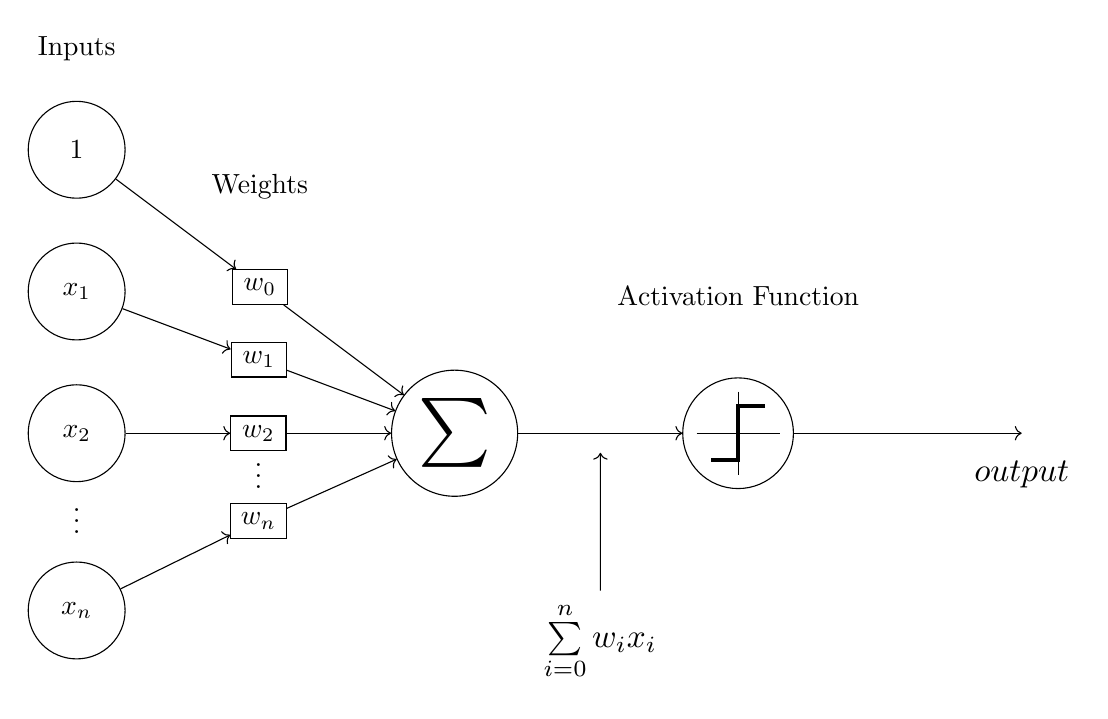
\begin{tikzpicture}[scale=1.2]
    % Draw input nodes
    \foreach \h [count=\hi ] in {$x_2$,$x_1$,$1$}{%
        \node[input] (f\hi) at (0,\hi*1.5cm-1.5 cm) {\h};
      }
    % Dot dot dot ... x_n
    \node[below=0.62cm] (idots) at (f1) {\vdots};
    \node[input, below=0.62cm] (last_input) at (idots) {$x_n$};
    % Draw summation node
    \node[functions] (sum) at (4,0) {\Huge$\sum$};
    % Draw edges from input nodes to summation node
    \foreach \h [count=\hi ] in {$w_2$,$w_1$,$w_0$}{%
          \path (f\hi) -- node[weights] (w\hi) {\h} (sum);
          \draw[->] (f\hi) -- (w\hi);
          \draw[->] (w\hi) -- (sum);
        }
    % Dot dot dot ... w_n
    \node[below=0.05cm] (wdots) at (w1) {\vdots};
    \node[weights, below=0.45cm] (last_weight) at (wdots) {$w_n$};
    % Add edges for last node and last weight etc
    \path[draw,->] (last_input) -- (last_weight);
    \path[draw,->] (last_weight) -- (sum);
    % Draw node for activation function
    \node[functions] (activation) at (7,0) {};
    % Place activation function in its node
    \begin{scope}[xshift=7cm,scale=1.25]
        \addaxes
        % flexible selection of activation function
        % \relu
        \stepfunc
    \end{scope}
    % Connect sum to activation function
    \draw[->] (sum) -- (activation) node (sum_eq) [midway, below=2cm, scale=1.2] {$\sum\limits_{i=0}^n w_ix_i$} node (sum_activation_midway) [midway, below] {};
    \path[draw,->] (sum_eq) -- (sum_activation_midway);
    \draw[->] (activation) -- ++(3,0) node (perceptron_output) [below=0.2cm, scale=1.2] {$output$};
    % Labels
    \node[above=1cm]  at (f3) {Inputs};
    \node[above=1cm] at (w3) {Weights};
    \node[above=1.5cm] at (activation) {Activation Function};
\end{tikzpicture}
\caption{Single-Layer Perceptron.\protect\footnotemark}
\label{fig:perceptron}
\end{figure}
%From: https://tex.stackexchange.com/questions/104334/tikz-diagram-of-a-perceptron


Thus, the Perceptron is a linear classifier, in other words, it is an algorithm that classifies input by separating two classes with a straight line. The learning algorithm used for adjusting the weights of the Perceptron can be summarized in the following steps:

\begin{enumerate}
    \item Start by initializing the vector of weights to random values.
    \item For each training sample \( x_i \), compute output \( \hat{y}_i \) with the current vector of weights.
    \item If the Perceptron makes an incorrect prediction, update the weights according to the following formula:
    \begin{equation}
        \theta_{i} = \theta_i - \lambda(\hat{y}_t-y_t)x_t
    \end{equation}
    where \( \lambda \) is the learning rate, \( \hat{y} \) is the predicted output and \( y \) is the actual output.
    \item Repeat steps from 2 to 4 for a fixed number of epochs or until the model converges. An epoch is one complete pass through the entire dataset.

\end{enumerate}

The convergence of the Perceptron is only guaranteed if the two classes are linearly separable. If the data is not linearly separable, the algorithm will not converge and the weights will oscillate indefinitely. The XOR Problem, introduced in the book Perceptrons \cite{rosenblatt1958perceptron}, is a classic example of a non-linearly separable problem, which consists in predicting the output of XOR logic gates. This problem illustrates the inability of the Perceptron to solve non-linearly separable problems. Figure \ref{fig:xor} shows a representation of the XOR problem, it can be seen that the two classes cannot be separated by a straight line.

\footnotetext{Adapted from \url{https://tex.stackexchange.com/questions/104334/tikz-diagram-of-a-perceptron}}

\begin{figure}[h]
\centering
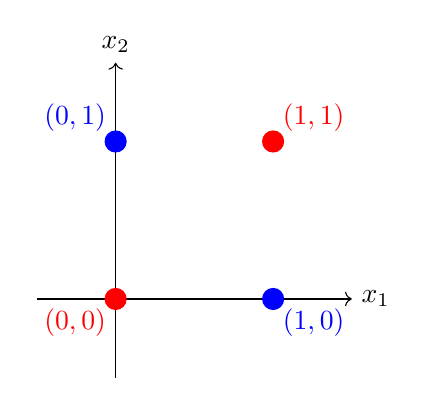
\begin{tikzpicture}[scale=2]
    % Axes
    \draw[->] (-0.5,0) -- (1.5,0) node[right] {$x_1$};
    \draw[->] (0,-0.5) -- (0,1.5) node[above] {$x_2$};
    
    % Points for Class 1 (0,1) and (1,0)
    \fill[blue] (0,1) circle (2pt) node[above left] {$(0,1)$};
    \fill[blue] (1,0) circle (2pt) node[below right] {$(1,0)$};
    
    % Points for Class 2 (0,0) and (1,1)
    \fill[red] (0,0) circle (2pt) node[below left] {$(0,0)$};
    \fill[red] (1,1) circle (2pt) node[above right] {$(1,1)$};

    % Labels for classes
    \node[blue] at (-0.5, 1.2){};
    \node[red] at (1.5, 1.2) {};

    % Grid lines for reference
    %\draw[dashed, gray] (0,0) grid (1,1);
    
    % Optional: Lines connecting points to form a square
    %\draw[gray] (0,0) -- (0,1) -- (1,1) -- (1,0) -- cycle;

\end{tikzpicture}
\caption{Graph representing the XOR problem with two classes. The colours of the dots represent their class.}
\label{fig:xor}
\end{figure}

\subsection{Multi-Layer Perceptron}

To address the limitations of the basic Perceptron, more advanced models have been developed. The most popular one is the Multi-Layer Perceptron (MLP), which consists of an input layer, one or more hidden layers and an output layer (see Figure \ref{fig:multilayer-perceptron}). The hidden layers enable the network to learn complex patterns between inputs and outputs.

% Figure of multi-layer perceptron
\begin{figure}[h]
	\centering
	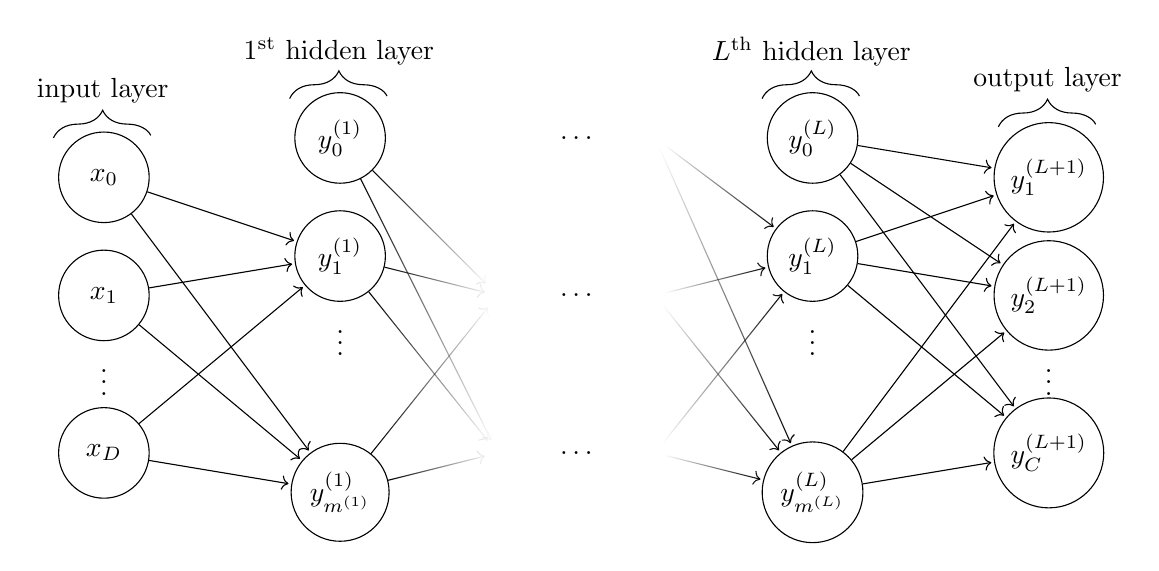
\begin{tikzpicture}[shorten >=1pt]
		\tikzstyle{unit}=[draw,shape=circle,minimum size=1.15cm]
		%\tikzstyle{hidden}=[draw,shape=circle,fill=black!25,minimum size=1.15cm]
		\tikzstyle{hidden}=[draw,shape=circle,minimum size=1.15cm]

		\node[unit](x0) at (0,3.5){$x_0$};
		\node[unit](x1) at (0,2){$x_1$};
		\node at (0,1){\vdots};
		\node[unit](xd) at (0,0){$x_D$};

		\node[hidden](h10) at (3,4){$y_0^{(1)}$};
		\node[hidden](h11) at (3,2.5){$y_1^{(1)}$};
		\node at (3,1.5){\vdots};
		\node[hidden](h1m) at (3,-0.5){$y_{m^{(1)}}^{(1)}$};

		\node(h22) at (5,0){};
		\node(h21) at (5,2){};
		\node(h20) at (5,4){};
		
		\node(d3) at (6,0){$\ldots$};
		\node(d2) at (6,2){$\ldots$};
		\node(d1) at (6,4){$\ldots$};

		\node(hL12) at (7,0){};
		\node(hL11) at (7,2){};
		\node(hL10) at (7,4){};
		
		\node[hidden](hL0) at (9,4){$y_0^{(L)}$};
		\node[hidden](hL1) at (9,2.5){$y_1^{(L)}$};
		\node at (9,1.5){\vdots};
		\node[hidden](hLm) at (9,-0.5){$y_{m^{(L)}}^{(L)}$};

		\node[unit](y1) at (12,3.5){$y_1^{(L+1)}$};
		\node[unit](y2) at (12,2){$y_2^{(L+1)}$};
		\node at (12,1){\vdots};	
		\node[unit](yc) at (12,0){$y_C^{(L+1)}$};

		\draw[->] (x0) -- (h11);
		\draw[->] (x0) -- (h1m);

		\draw[->] (x1) -- (h11);
		\draw[->] (x1) -- (h1m);

		\draw[->] (xd) -- (h11);
		\draw[->] (xd) -- (h1m);

		\draw[->] (hL0) -- (y1);
		\draw[->] (hL0) -- (yc);
		\draw[->] (hL0) -- (y2);

		\draw[->] (hL1) -- (y1);
		\draw[->] (hL1) -- (yc);
		\draw[->] (hL1) -- (y2);

		\draw[->] (hLm) -- (y1);
		\draw[->] (hLm) -- (y2);
		\draw[->] (hLm) -- (yc);

		\draw[->,path fading=east] (h10) -- (h21);
		\draw[->,path fading=east] (h10) -- (h22);
		
		\draw[->,path fading=east] (h11) -- (h21);
		\draw[->,path fading=east] (h11) -- (h22);
		
		\draw[->,path fading=east] (h1m) -- (h21);
		\draw[->,path fading=east] (h1m) -- (h22);
		
		\draw[->,path fading=west] (hL10) -- (hL1);
		\draw[->,path fading=west] (hL11) -- (hL1);
		\draw[->,path fading=west] (hL12) -- (hL1);
		
		\draw[->,path fading=west] (hL10) -- (hLm);
		\draw[->,path fading=west] (hL11) -- (hLm);
		\draw[->,path fading=west] (hL12) -- (hLm);
		
		\draw [decorate,decoration={brace,amplitude=10pt},xshift=-4pt,yshift=0pt] (-0.5,4) -- (0.75,4) node [black,midway,yshift=+0.6cm]{input layer};
		\draw [decorate,decoration={brace,amplitude=10pt},xshift=-4pt,yshift=0pt] (2.5,4.5) -- (3.75,4.5) node [black,midway,yshift=+0.6cm]{$1^{\text{st}}$ hidden layer};
		\draw [decorate,decoration={brace,amplitude=10pt},xshift=-4pt,yshift=0pt] (8.5,4.5) -- (9.75,4.5) node [black,midway,yshift=+0.6cm]{$L^{\text{th}}$ hidden layer};
		\draw [decorate,decoration={brace,amplitude=10pt},xshift=-4pt,yshift=4pt] (11.5,4) -- (12.75,4) node [black,midway,yshift=+0.6cm]{output layer};
	\end{tikzpicture}
	\caption[Network graph for a $(L+1)$-layer perceptron.]{Network graph of a $(L+1)$-layer perceptron with $D$ input units and $C$ output units. The $l^{\text{th}}$ hidden layer contains $m^{(l)}$ hidden units.\protect\footnotemark}
	\label{fig:multilayer-perceptron}
\end{figure}
%From https://github.com/davidstutz/latex-resources/blob/master/tikz-multilayer-perceptron/multilayer-perceptron.tex


In an MLP, each neuron in a given layer is fully connected to the neurons in the previous and subsequent layers, meaning that every neuron in one layer receives inputs from all the neurons in the previous layer and sends its output to all neurons in the next layer. The equation defined by a MLP with $L$ layers can be expressed as:
\footnotetext{Obtained from \url{https://github.com/davidstutz/latex-resources/blob/master/tikz-multilayer-perceptron/multilayer-perceptron.tex}}
%
\begin{equation}
    y_i^l = g\left(\sum_{j=0}^{M_{l-1}}\theta_{ij}^l  y_j^{l-1}\right), \text{  }1 \leq i \leq M_l, 2 \leq l \leq L
\end{equation}
%
\begin{equation}
    y_i^1 = g\left(\sum_{j=0}^{M_0} \theta_{ij}^1x_j\right), \text{   } 1 \leq i \leq M_1
\end{equation}
%
where $y_i^l $ is the output of the $i^{th}$ node in layer $l$; $\theta_{ij}^l$ denotes the weight of the connection that goes from the $j^{th}$ node of layer $l-1$ to the $i^{th}$ of layer $l$; and $M_l$ is the dimension of layer $l$.

Activation functions \( g(\cdot)\) introduce non-linearity into the MLP and allow it to deal with non-linear decision boundaries. Some examples of activation functions are the ReLU \cite{agarap2018relu}, the Sigmoid or the hyperbolic tangent.

The learning process of an MLP is typically carried out using the backpropagation algorithm combined with an optimization technique such as gradient descent. The formula for updating the weights of the network can be expressed as:
%
\begin{equation}
    \Delta \theta_{ij}^l=-\lambda \frac{\partial L(\theta)}{\partial \theta_{ij}^l}
\end{equation}

% where \( L(\theta) \) is the loss function we want to optimize. The choice of this loss function depends on the nature of the task.

% In classification problems with C classes, the most common is the Cross-Entropy Loss. This function measures the difference between two probability distributions.

% \begin{equation}
%     L(\theta) = - \sum_{c=1}^Cy_clog(\hat{y}_c)
% \end{equation}

% On the other hand, in regression problems the most common loss functions are the Mean Squared Error (MSE) and the Mean Absolute Error (MAE).

% \begin{equation}
%     MSE = \frac{1}{N} \sum_{i=1}^{N} (y_i - \hat{y}_i)^2
% \end{equation}

% \begin{equation}
%     MAE = \frac{1}{N} \sum_{i=1}^{N} |y_i - \hat{y}_i|
% \end{equation}

\subsection{Recurrent Neural Networks}

An NN without loops, where the information can only flow in one direction forming a directed acyclic graph (DAG), is known as Feedforward NN (FNN). The main limitation of this kind of networks is their inability to maintain context or memory of past inputs, as each input is processed independently. To overcome this problem, Recurrent Neural Networks (RNNs) were introduced. This kind of NN translates an input sequence space into an output sequence space in a manner that retains state information. Specifically, the prediction $y_t$ at instant $t$ is influenced by both the input $x_t$ and the system's current hidden state $h_t$, which is updated over time, as the sequence is processed. Figure \ref{fig:rnn_structure} shows a diagram of an RNN.


%maps from an input space of sequences to an output space of sequences in a stateful way. That is, the prediction \( y_t \) at instant \( t \) depends not only on the input \( x_t \), but also on the current hidden state of the system \( h_t \), which is updated over time, as the sequence is processed. 

% Figure RNN
\begin{figure}[h]
    \centering
    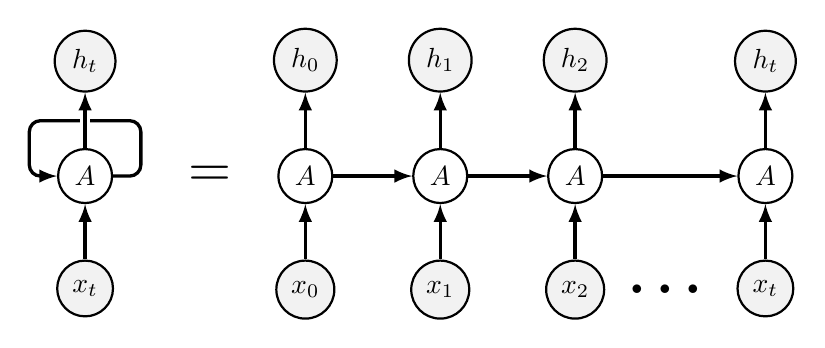
\begin{tikzpicture}[item/.style={circle,draw,thick,align=center},
    itemc/.style={item,on chain,join}]
        \begin{scope}[start chain=going right,nodes=itemc,every join/.style={-latex,very thick},local bounding box=chain]
            \path node (A0) {$A$} 
                  node (A1) {$A$} 
                  node (A2) {$A$} 
                  node[xshift=2em] (At) {$A$};
        \end{scope}
        \node[left=1em of chain,scale=2] (eq) {$=$};
        \node[left=2em of eq,item] (AL) {$A$};
        \path (AL.west) ++ (-1em,2em) coordinate (aux);
        \draw[very thick,-latex,rounded corners] (AL.east) -| ++ (1em,2em) -- (aux) |- (AL.west);
        \foreach \X in {0,1,2,t} {
            \draw[very thick,-latex] (A\X.north) -- ++ (0,2em) node[above,item,fill=gray!10] (h\X) {$h_\X$};
            \draw[very thick,latex-] (A\X.south) -- ++ (0,-2em) node[below,item,fill=gray!10] (x\X) {$x_\X$};
        }
        \draw[white,line width=0.8ex] (AL.north) -- ++ (0,1.9em);
        \draw[very thick,-latex] (AL.north) -- ++ (0,2em) node[above,item,fill=gray!10] {$h_t$};
        \draw[very thick,latex-] (AL.south) -- ++ (0,-2em) node[below,item,fill=gray!10] {$x_t$};
        \path (x2) -- (xt) node[midway,scale=2,font=\bfseries] {\dots};
    \end{tikzpicture}
    \caption{Illustration of an RNN structure with hidden states and inputs.\protect\footnotemark}
    \label{fig:rnn_structure}
\end{figure}
%https://tex.stackexchange.com/questions/494139/how-do-i-draw-a-simple-recurrent-neural-network-with-goodfellows-style
\footnotetext{Obtained from \url{https://tex.stackexchange.com/questions/494139/how-do-i-draw-a-simple-recurrent-neural-network-with-goodfellows-style}}

The main drawback of RNNs is that they struggle to capture long-term dependencies in input sequences. During backpropagation, gradients are propagated from the last neuron all the way to the first one. The repeated multiplication of gradients through the hidden states can result in gradient vanishing or exploding, that is, gradients can become extremely small or large.

In order to tackle these limitations, the Long-Short Term Memory (LSTM) networks were introduced \cite{hochreiter1997long}. They are a type of RNN that introduce a more sophisticated architecture enabling them to maintain information over longer periods, making them particularly effective for tasks involving sequential data, such as NLP.

LSTM units typically consist of a memory cell along with an input gate, output gate, and forget gate (see Figure \ref{fig:lstm_architecture}). The memory cell retains values over time, while the three gates manage the information flow in and out of the cell. The input gate is responsible for deciding what new information is stored in the cell's current state. Conversely, the forget gate determines what information is eliminated from the cell state. Lastly, the output gate regulates what information from the cell state is used as the output.

%Figure of LSTM unit 
\begin{figure}[ht]
    \centering
    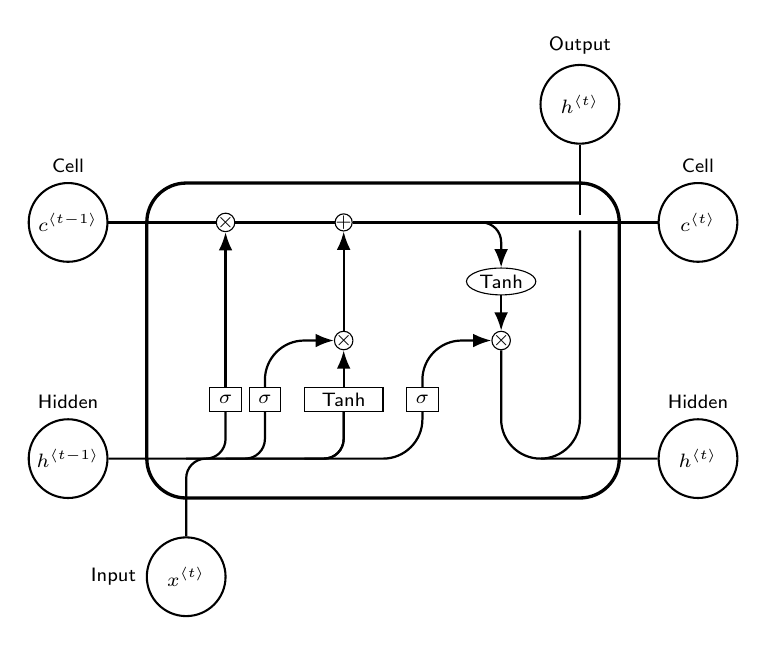
\begin{tikzpicture}[
        font=\sf \scriptsize,
        >=LaTeX,
        cell/.style={
            rectangle, 
            rounded corners=5mm, 
            draw,
            very thick,
        },
        operator/.style={
            circle,
            draw,
            inner sep=-0.5pt,
            minimum height =.2cm,
        },
        function/.style={
            ellipse,
            draw,
            inner sep=1pt
        },
        ct/.style={
            circle,
            draw,
            line width = .75pt,
            minimum width=1cm,
            inner sep=1pt,
        },
        gt/.style={
            rectangle,
            draw,
            minimum width=4mm,
            minimum height=3mm,
            inner sep=1pt
        },
        mylabel/.style={
            font=\scriptsize\sffamily
        },
        ArrowC1/.style={
            rounded corners=.25cm,
            thick,
        },
        ArrowC2/.style={
            rounded corners=.5cm,
            thick,
        },
    ]

    % Drawing starts here
    \node [cell, minimum height =4cm, minimum width=6cm] {}; 

    % Draw inputs named ibox#
    \node [gt] (ibox1) at (-2,-0.75) {$\sigma$};
    \node [gt] (ibox2) at (-1.5,-0.75) {$\sigma$};
    \node [gt, minimum width=1cm] (ibox3) at (-0.5,-0.75) {Tanh};
    \node [gt] (ibox4) at (0.5,-0.75) {$\sigma$};

   % Draw operators   named mux# , add# and func#
    \node [operator] (mux1) at (-2,1.5) {$\times$};
    \node [operator] (add1) at (-0.5,1.5) {+};
    \node [operator] (mux2) at (-0.5,0) {$\times$};
    \node [operator] (mux3) at (1.5,0) {$\times$};
    \node [function] (func1) at (1.5,0.75) {Tanh};

    % Draw External inputs, named as basis c,h,x
    \node[ct, label={[mylabel]Cell}] (c) at (-4,1.5) {\empt{c}{t-1}};
    \node[ct, label={[mylabel]Hidden}] (h) at (-4,-1.5) {\empt{h}{t-1}};
    \node[ct, label={[mylabel]left:Input}] (x) at (-2.5,-3) {\empt{x}{t}};

    % Draw External outputs, named as basis c2,h2,x2
    \node[ct, label={[mylabel]Cell}] (c2) at (4,1.5) {\empt{c}{t}};
    \node[ct, label={[mylabel]Hidden}] (h2) at (4,-1.5) {\empt{h}{t}};
    \node[ct, label={[mylabel]Output}] (x2) at (2.5,3) {\empt{h}{t}};
    
% Start connecting all.
    %Intersections and displacements are used. 
    % Drawing arrows    
    \draw [ArrowC1] (c) -- (mux1) -- (add1) -- (c2);

    % Inputs
    \draw [ArrowC2] (h) -| (ibox4);
    \draw [ArrowC1] (h -| ibox1)++(-0.5,0) -| (ibox1); 
    \draw [ArrowC1] (h -| ibox2)++(-0.5,0) -| (ibox2);
    \draw [ArrowC1] (h -| ibox3)++(-0.5,0) -| (ibox3);
    \draw [ArrowC1] (x) -- (x |- h)-| (ibox3);

    % Internal
    \draw [->, ArrowC2] (ibox1) -- (mux1);
    \draw [->, ArrowC2] (ibox2) |- (mux2);
    \draw [->, ArrowC2] (ibox3) -- (mux2);
    \draw [->, ArrowC2] (ibox4) |- (mux3);
    \draw [->, ArrowC2] (mux2) -- (add1);
    \draw [->, ArrowC1] (add1 -| func1)++(-0.5,0) -| (func1);
    \draw [->, ArrowC2] (func1) -- (mux3);

    %Outputs
    \draw [-, ArrowC2] (mux3) |- (h2);
    \draw (c2 -| x2) ++(0,-0.1) coordinate (i1);
    \draw [-, ArrowC2] (h2 -| x2)++(-0.5,0) -| (i1);
    \draw [-, ArrowC2] (i1)++(0,0.2) -- (x2);

    \end{tikzpicture}
    \caption{Architecture of an LSTM unit.\protect\footnotemark}
    \label{fig:lstm_architecture}
\end{figure}

%\footnotetext{Obtained from \url{https://tex.stackexchange.com/questions/701738/gru-unit-cell-changing-from-lstm-to-gru}}

\section{Transformers}

%The transformer architecture represent a revolutionary architecture in the field of deep learning, particularly in NLP. It has 

Transformers represent a revolution in the field of deep learning, particularly in NLP, by introducing a powerful architecture that excels in handling sequential data and capturing long-range dependencies. Unlike traditional RNN and their variants, transformers rely on self-attention mechanisms that allow them to process all elements of a sequence simultaneously, rather than sequentially. This innovation enables transformers to model complex patterns and relationships within data.

Since they were initially used for MT, the original Transformer architecture consists of an encoder-decoder structure (see Figure \ref{fig:transformer}). The encoder takes a sequence as input and transforms it into a state with fixed shape. This state is passed to the decoder, which maps the encoded representation of the input to an output sequence.

% Figure of original Transformer
\begin{figure}[h]
    \centering
    \includegraphics[width=0.5\linewidth]{figures/transformer.pdf}
    \caption{Original Transformer architecture. Extracted from \cite{vaswani2017attention}.}
    \label{fig:transformer}
\end{figure}


\subsection{Self-Attention}

Self-attention, also known as scaled dot-product attention, is the mechanism that allows the Transformer to capture long-range dependencies within data. The key intuition behind using self-attention for sequence analysis lies in its ability to assign different importance weights to different parts of the input sequence. The self-attention process can be described as follows:

\begin{enumerate}
    \item Input embeddings: Each input token is first embedded into a continuous vector space.
    
    \item Query, Key and Value vectors: The input embedding \( x_i \), for each word \( i \), is linearly transformed into the query (\(Q\)), key (\(K\)) and value (\(V\)) vectors using learned weight matrices \(W_Q\), \(W_K\), \(W_V\).

    \item Attention scores: The attention score between a pair of tokens is computed as the dot product of their query and key vectors. This score is then scaled by the square root of the dimension of the key vectors, \(\sqrt{d_k}\) and passed through a softmax function to obtain attention weights.

    \item Weighted sum: Finally, the output for each query is calculated as the weighted sum of the value vectors, where the weights are the attention scores computed in the previous step. 
\end{enumerate}

Mathematically, the self-attention mechanism is expressed as follows:
%
\begin{equation}
\text{Attention}(Q, K, V) = \text{softmax}\left(\frac{QK^T}{\sqrt{d_k}}\right)V
\end{equation}

\footnotetext{Obtained from \url{https://tex.stackexchange.com/questions/701738/gru-unit-cell-changing-from-lstm-to-gru}}

\subsection{Multi-Head Attention}

In a single attention mechanism, each position in the input sequence attends to all other positions, creating a single context vector for each position. While this approach is powerful, it can be limiting because it compresses all the information into a single vector.

Multi-head attention addresses this limitation by employing multiple attention mechanisms, or "heads," in parallel. Each head operates on a different linear projection of the queries, keys, and values, allowing the model to capture diverse features and dependencies from various subspaces of the input data. Therefore, the main idea behind multi-head attention is to enable the model to focus on different parts of the input simultaneously and from different perspectives.

Each head has its own set of learned weight matrices \(W_Q\), \(W_K\) and \(W_K\) and performs scaled dot-product attention independently. Then, the outputs of all attention heads are concatenated and then linearly transformed, using another weight matrix \(W_O\), to produce the final output:
%
\begin{equation}
    \text{MultiHead}(Q, K, V) = \text{Concat}(\text{head}_1, \text{head}_2, \ldots, \text{head}_h)W^O
\end{equation}
%
where each head output is computed as:
%
\begin{equation}
    \text{head}_i = \text{Attention}(QW_i^Q, KW_i^K, VW_i^V)
\end{equation}

\subsection{Transformer Architecture}
\label{subseq:transformer_arch}

The original Transformer model is composed of two main parts: the encoder and the decoder. Both are built upon stacks of identical layers, but their roles and compositions differ slightly.

The encoder's primary function is to process the input sequence and generate a continuous representation of it. Each encoder layer consists of two sub-layers. The first is a multi-head self-attention mechanism, while the second is a position-wise fully connected FNN, which consists of two linear transformations with a ReLU activation in between. The formula of the output produced by the FNN can be expressed as:
%
\begin{equation}
    \text{FNN}= \max(0, xW_1 + b_1)W_2 + b_2
\end{equation}

Additionaly, both sub-layers are wrapped with residual connections and layer normalization to facilitate the training process.

The decoder, on the other hand, generates the output sequence by attending to both the encoder's output and the previous tokens in the output sequence. In addition to the two sub-layers present in each encoder layer, the decoder includes a third sub-layer that performs multi-head attention over the output of the encoder stack. Moreover, the decoder uses masked selft-attention to ensure that predictions for a given position depend only on the previous outputs and not on any future token.

\subsection{Word Embeddings and Positional Encoding}

Word embeddings (WE) are the first step in transforming the raw input tokens into a format that can be processed by the Transformer. They convert discrete tokens, such as words or subwords, into continuous vectors of fixed dimensions. This allows the model to capture semantic meanings and relationships between tokens. 

However, embeddings do not contain information about the order of the tokens in the sequence. Transformers, unlike RNNs, do not process tokens sequentially. Therefore, positional encoding (PE) is used to inject information about the position of each token $x$ in the sequence. This is accomplished by adding a vector to each token embedding containing the positional information:

\begin{equation}
    \text{Embedding(x)} = WE + PE
\end{equation}

Positional encodings can be learnt or fixed \cite{gehring2017convolutional}. The authors of the original Transformer considered a fixed approach that uses sinusoidal functions with different frequencies:

\begin{equation}
    \text{PE}_{(pos, 2i)} = \sin\left(\frac{pos}{10000^{\frac{2i}{d_{\text{model}}}}}\right)
\end{equation}

\begin{equation}
    \text{PE}_{(pos, 2i+1)} = \cos\left(\frac{pos}{10000^{\frac{2i}{d_{\text{model}}}}}\right)
\end{equation}

where \(pos\) is the position of the token in the sequence, \(i\) is the dimension index and \(d_{model}\) is the dimension of the model embeddings.

The fusion of WE and PE unlocks the Transformer's ability to comprehend sequences. These mechanisms allow transformers to leverage both the semantic meaning and the order of tokens, facilitating their application to a wide range of NLP tasks, such as MT, sentiment analysis or text generation.

\section{Large Language Models}

The field of AI has been revolutionized by the emergence of foundation models. Foundation models \cite{bommasani_foundation}, a term coined by the Stanford Institute for Human-Centered AI (HAI), refer to large-scale models trained on broad data that can be adapted to a wide range of downstream tasks. 

LLMs are a subset of foundation models, primarily focused on NLP. These models are usually based on the Transformer architecture and are designed to understand and generate human language with a high degree of fluency and coherence. LLMs are characterized by their massive scale, both in terms of the volume of training data and their number of parameters.

Language is a prominent ability in humans that allows them to express and communicate. Machines, however, do not have that inherent ability of understanding and communicating in the form of human language. For this reason, language modeling (LM), a critical component of NLP, is one of the most active areas of research within the vast field of AI. In general, LM seeks to estimate the generative likelihood of word sequences, such that missing tokens are predicted based on the predicted probabilities.


%aims to model the generative likelihood of word sequences, so as to predict the probabilities of future (or missing) tokens \cite{zhao2023surveyllm}.

The evolution of language models has been marked by significant advancements. It began with statistical language models (SLMs), which utilized statistical approaches to predict the likelihood of word sequences based on observed frequencies in training data. Following SLMs, neural language models (NLMs) emerged, leveraging neural network architectures to capture complex linguistic patterns. NLMs are trained on task-specific data so as to solve specific tasks. In contrast, pre-trained language models (PLMs) are task-agnostic, meaning that they are normally trained to solve general NLP tasks. Their training and inference follow a pre-training and fine-tuning approach, where models first undergo a self-supervised training on extensive text corpora comprising typical NLP problems and are then fine-tuned with a small amount of task-specific labeled data. 


NLMs are task-specific models, since they are trained on task-specific data. Pre-trained language models (PLMs), unlike NLMs, are task-agnostic. Their training and inference follow the pre-training and fine-tuning paradigm, where models are trained in a self-supervised setting on a large corpus of text for general NLP tasks, and then fine-tuned to specific tasks using small amounts of labeled task-specific data. Finally, LLMs appeared as the latest milestone in the field of NLP. They mainly refer to transformer-based NLMs that are trained on massive text data and contain tens to hundreds of billions of parameters. 

\subsection{Types of architecture}

LLMs can be broadly categorized based on their architecture into three main types:

\begin{itemize}
    \item Encoder-decoder: They are also known as sequence-to-sequence models (Seq2Seq). These models follow the original Transformer architecture presented in Section \ref{subseq:transformer_arch} and they are designed for transforming an input sequence into an output sequence. Examples of this type of model include Google's T5\cite{raffel2020t5} and BART \cite{lewis2019bart}.

    \item Encoder-only: These models are primarily used for tasks that require a deep understanding of the input text, such as text classification, sentiment analysis or named entity recognition. A popular example of encoder-only models is BERT (Bidirectional Encoder Representations from Transformers) \cite{devlin2018bert}. BERT is designed to understand the context of words in a sentence by considering both the left and right context, making it highly effective for tasks that require a nuanced understanding of language.

    \item Decoder-only: They are also know as autoregressive models. These models generate sequences by predicting the next token in the sequence based on the previous tokens, making them suitable for text generation tasks. Prominent examples of decoder-only models are GPT \cite{Radford2018gpt1} \cite{Radford2019gpt2} \cite{brown2020gpt3} \cite{achiam2023gpt4} and Llama \cite{touvron2023llama} \cite{touvron2023llama2} families developed by OpenAI and Meta, respectively. In recent years, this type of models has stood out above the rest, to such an extent that they have practically taken over the term "LLM".

    \item Mixture of Experts (MoE): These models are a variant of Transformer architecture that consists of a certain number of neural networks, known as experts, and a gate network or router, which determines which tokens are sent to which expert. This selective activation of experts allows MoEs to allocate computational resources more effectively, focusing on relevant experts for specific inputs while keeping the rest inactive. These type of models gained popularity with the release of Mistral 7x8B \cite{jiang2024mixtral}.
\end{itemize}

\subsection{Scalable Training Techniques}

With the increasing trend of model and data sizes, the computational resources needed for training LLMs are also increasing. This hinders the training and deployment of LLMs to individuals or small companies with low computational resources. The main issues to be resolved are: increasing training throughput and loading larger models into available GPUs. To address the above two challenges, some approaches have been developed, such as 3D parallelism and ZeRO.

3D parallelism is actually a combination of three parallel training techniques that allow the training of LLMs using multiple devices:

\begin{itemize}
    \item Data parallelism: Each device contains a copy of the model, including model parameters and optimizer states. Subsequently, the training corpus is partitioned among all the devices, with each device handling its allocated data independently. Gradients are computed locally on each device and will be further aggregated to obtain the gradients of the whole batch, ensuring synchronized updates to all the copies of the model.
    
    %Then, the training corpus is distributed over all the devices in such a way that each device processes only the data assigned to it and obtains the gradients, which will be further aggregated to obtain the gradients of the whole batch and update the model parameters in all GPUs.

    \item Pipeline parallelism: The different layers of an LLM are distributed among multiple devices. In the case of Transformer-based models, consecutive layers are allocated to the same device in order to minimize the overhead of transmitting the computed gradients or states among devices.

    \item Tensor parallelism: This technique distributes the computations of the model across multiple devices by splitting tensors into non-overlapping pieces. These tensor shards are processed in parallel and later combined to obtain the final result.
\end{itemize}

ZeRO \cite{rajbhandari2020zero} technique, on the other hand, aims to solve the data redundancy problem present in data parallelism. As previously mentioned, data parallelism replicates the model parameters, optimizer states and model gradients across all the devices. ZeRO aims to tackle this issue by partitioning the data across multiple devices, reducing memory consumption while retaining low communication costs and high computational granularity.
 
Additionally to these parallelization techniques, there are other common approaches that are crucial for optimizing LLMs. Traditionally, NNs used to be trained using FP32, but with the rapidly increasing number of parameters in LLMs, training with FP32 is becoming very costly in time and memory. In order to tackle this issue, mixed-precision training \cite{micikevicius2017mixed} was introduced, which stores the model weights in FP32 for retaining accuracy, but uses FP16 for performing computations during training and inference. Another technique that allows for efficient training of LLMs is quantization, which focuses on converting the parameters and activations of the model from high-precision formats, such as FP32, to lower-precision representations, such as 8-bit \cite{dettmers2022int8} or 4-bit integers. This conversion drastically reduces the model's memory footprint and computational requirements while maintaining performance close to high-precision formats, making it more feasible to deploy LLMs on resource-constrained scenarios. These techniques are crucial in making LLMs more accessible and efficient for practical applications.

%TODO: MENTION FSDP

\subsection{Decoding strategies}

Once the LLM has been pre-trained, the process of generating the output text is known as decoding. Text generation starts by converting the input prompt into smaller parts (tokens), this process is known as tokenization. Then, the model processes these tokens and generates logits, which are passed through a softmax function to obtain the probability of each token of the vocabulary. The final step consists in selecting the next token based on the computed probabilities following a certain decoding strategy. Different decoding strategies have been proposed, being the following the most popular ones:

\begin{itemize}
    \item Greedy search: This is the simplest and most straightforward strategy. At each generation step, the token with the highest probability is selected. Although it is fast, this strategy can overlook potentially better sequences that could arise from selected tokens with slightly lower probabilities. 

    \item Beam search: This strategy considers multiple potential token sequences at each step, keeping track of the $N$ most likely tokens, with $N$ indicating the beam size. This process continues until either the maximum sequence length is reached or an end-of-sequence token is generated. The final output corresponds to the beam with the highest cumulative probability. Although beam search is more likely to generate coherent and contextually appropriate text than greedy search, it requires significantly more computational resources due to the simultaneous evaluation of several possible sequences.

    \item Top-k sampling: Limits the selection pool to the top-k most likely tokens. The probabilities of these top-k tokens are re-normalized so they sum to 1. Finally, one of these tokens is randomly selected based on the re-normalized probabilities previously computed. 

    \item Top-p sampling: Unlike top-k sampling, which selects the top-k tokens based on their probabilities, top-p sampling dynamically selects the smallest subset of tokens whose cumulative probability exceeds a threshold \(p\). From this set, a token is randomly chosen based on the re-normalized probabilities of the tokens. This method allows for greater adaptability and context sensitivity in the decoding process, since the number of candidate tokens is dynamically adjusted at each generation step.
    %https://deci.ai/blog/from-top-k-to-beam-search-llm-decoding-strategies/
\end{itemize}

\subsection{Prompting}

Prompting refers to the process of providing an initial input or query to an LLM to guide its text generation or task performance. LLMs can be prompted in various prompt setups. Below, we will introduce the most used ones:

\begin{itemize}
    \item Zero-shot prompting: The prompt does not contain any examples or demonstrations. Large scale training makes these models capable of answering queries never seen before without seeing any example.

    \item In-context learning (ICL): The prompt contains some input-output demonstration pairs. This technique, also known as few-shot learning, allows pre-trained LLMs to address new tasks without fine-tuning the model. ICL's efficacy was demonstrated in the GPT-3 original paper \cite{brown2020gpt3}.

    \item Chain-of-thought (CoT): This prompting method helps LLMs perform complex reasoning tasks by breaking down the problem into a series of intermediate steps, thus guiding the model towards the final answer \cite{wei2022chain}.

    \item Self consistency: Presented in \cite{wang2022self}, it aims to improve CoT performance. The idea is to sample multiple diverse reasoning paths and selecting the most consistent and coherent answers.  

    \item Tree of thought (ToT): This prompting technique tries to emulate human-like trial and error decision-making \cite{long2023ToT}. It involves creating a hierarchical structure where each branch represents a reasoning path consisting of intermediate steps towards the solution of the problem. The model is able to self-evaluate the progress to determine the next step by exploring the generated intermediate steps through lookahead and backtracking \cite{yao2024ToT}.
\end{itemize}

\subsection{Parameter Efficient Fine-Tuning}

In recent years, the number of parameters in LLMs has increased drastically. Therefore, traditional fine-tuning, which involves updating all the parameters of a pre-trained model, has become very costly in time and memory. Parameter-efficient fine-tuning (PEFT) \cite{han2024peft} techniques aim to address these limitations by updating only a small subset of the model's parameters, thus reducing the computational cost while maintaining a performance comparable to full-parameter fine-tuning. A prominent technique in the realm of PEFT is \textbf{Low-Rank Adaptation (LoRA)}\cite{hu2021lora}.


The core idea behind LoRA is that large pre-trained models possess a "low intrinsic dimension", this means that the full parameter space can be projected to a smaller dimensional space. Lying on this idea, LoRA assumes that the weight updates produced during fine-tuning can be also represented by a low-rank matrix. This insight enables LoRA to achieve faster training times and lower memory usage while producing more compact model weights that are easier to store and share. In practical terms, LoRA modifies a pre-trained weight matrix $W_0 \in R^{d \times k}$ by adding a low-rank update $\Delta W$. This update is expressed as the product of two smaller matrices, $B \in R^{d \times r}$ and $ A \in R^{r \times k}$, with $r$ being significantly smaller than both $d$ and $k$. Thus, the update of the pre-trained weights can be expressed as $W_0 + \Delta W = W_0 + BA$. During the fine-tuning process, the original weights $W_0$ are frozen and only $A$ and $B$ are trained. Typically, $A$ is initialized using a random Gaussian distribution, while $B$ is initialized with zeros, ensuring that $\Delta W = BA$ is zero at the start of training. In the forward pass, the input is multiplied by both $W_0$ and $\Delta W$, which are then summed coordinate-wise, as shown in Figure \ref{fig:lora}. Additionally, $\Delta W$ is scaled by a factor of $\frac{\alpha}{r}$, where $\alpha$ is a scaling factor:
%
\begin{equation}
    h = W_0x + \Delta Wx = W_0x + \frac{\alpha}{r} BAx
\end{equation}



%LoRA extends this idea and hypothesize that the difference between pre-trained and fine-tuned weights also 


%LoRA is based on a crucial insight that the difference between fine-tuned and pre-trained weights often exhibits "low intrinsic rank", this means that it can be approximated well by a low rank matrix. Therefore, training with LoRA is much faster, memory-efficient, and produces smaller model weights that are easier to store and share. Specifically, for a pre-trained weight matrix $W_0 \in R^{d \times k}$, its update is represented by a low rank decomposition $W_0 + \Delta W = W_0 + BA$, where $B \in R^{d \times r}$, $ A \in R^{r \times k}$, and the rank $r \ll \min (d,k).$ During training, $W_0$ is frozen and does not receive gradient updates, while A and B contain trainable parameters. Both $W_0$ and $\Delta W = BA$ are multiplied by the same input and their output vectors are then summed coordinate-wise.

%Usually, a random Gaussian initialization is used for $A$, and zero initialization for $B$, so $\Delta W = BA$ is zero at the beginning of training. Then, $\Delta W$ is scaled by $ \frac{\alpha}{r}$, where $\alpha$ is a scaling factor. The forward pass can be expressed as: 


It is worth mentioning that LoRA can be applied to any subset of weight matrices in an NN to reduce the number of trainable parameters. When applied to a Transformer, LoRA is often focused on adapting the attention weights $(W_q, W_k, W_v, W_o)$, while FNN weights are kept frozen. 

\begin{figure}[h]
    \centering    \includegraphics[width=0.5\linewidth]{lora.pdf}
    \caption{LoRA architecture. Extracted from \cite{hu2021lora}.}
    \label{fig:lora}
\end{figure}


%The core idea behind LoRA is to decompose the weight updates during fine-tuning into low-rank matrices. This decomposition allows for capturing task-specific knowledge with fewer parameters. In a typical NN, the weight matrix is a high-dimensional tensor. Instead of fine-tuning the entire weight matrix, LoRA introduces two low-rank matrices, A and B, such that the updated weight matrix W' is given 

\section{Machine Translation}

The journey of MT began in the mid-20th century with the advent of the first computers. The earliest attempts date back to the 1950s and were driven by the need for automated translation during Cold War. In 1954, IBM and Georgetown University conducted the Georgetown-IBM experiment \cite{hutchins-2004-georgetown}, which successfully translated 60 Russian sentences into English. Although limited in scope, this experiment demonstrated the potential of computers to perform linguistic tasks.

These early translation systems relied on rule-based methods (RBMT), generating translations by applying syntactic and grammatical rules to convert sentences from the source language to the target language. Linguists and computer scientists collaborated to develop extensive sets of linguistic rules and bilingual dictionaries. While these systems demonstrated successes, they struggled with idiomatic expressions and context-dependent meanings.

The next significant leap in MT came with the introduction of Statistical Machine Translation (SMT) \cite{brown1990smt} in the 1990s by IBM researchers. The core idea behind SMT was to treat translation as a probabilistic process, where the goal is to find the most likely translation for a given source sentence based on probabilities derived from large bilingual corpora. SMT systems segmented sentences into smaller units called phrases, which were then matched and translated based on their probability distributions. Unlike RBMT, SMT does not require developers to manually input rules for each language. While SMT significantly improved translation quality and scalability compared to RBMT approaches, it still had its limitations. SMT struggled with long-range dependencies, context understanding and the need for extensive parallel corpora.

The advent of deep learning and NNs in the 2010s revolutionized the field of MT with the rise of Neural Machine Translation (NMT). NMT systems make use of NNs to learn the mapping from source to target language in an end-to-end manner. Unlike SMT, which relies on separate components for translation and language modeling, NMT integrates both of these processes into a single NN architecture. NMT models are typically based on a encoder-decoder structure with RNNs \cite{sutskever2014seq2seq}, often enhanced with attention mechanisms. The encoder processes the input sequence, converting it into a fixed-length context vector that encapsulates the semantic meaning of the source text. The decoder then generates the translated sequence, word by word, using the context vector. The attention mechanism, introduced in 2014 \cite{bahdanau2014attention}, allows the model to dynamically focus on different parts of the input sequence during the translation process, significantly improving translation quality.

The introduction of the Transformer architecture marked another milestone in MT. Transformers, with their self-attention mechanism and parallel processing capabilities, enabled the training of even more powerful and efficient NMT models, and eliminated the need for recurrent structures, allowing for faster training and inference times. Currently, the MT models reporting the best results are those based on the original Transformer architecture.

The development of the Transformer not only enhance MT but also paved the way for the rising of LLMs, characterized by their large number of parameters as well as the massive datasets used in their training. LLMs excel in a variety of NLP tasks, this is why they are starting to be used for MT, exhibiting impressive results. The results of the WMT-23 shared task \cite{freitag2023results} indicated that GPT-4 with 5-shots can surpass models specifically designed for MT. 

%TO-DO: EXTEND TRANSFORMERS AND MENTION LLMs

\subsection{Evaluation Metrics}

Evaluating the quality of MT systems is crucial but poses several challenges. The best way to measure the quality of these systems is to get them evaluated by professional translators, who give a score for each translated sentence. However, human evaluation is usually unfeasible since it is costly and requires significant human labor. To overcome this, several automatic evaluation metrics have been postulated. These metrics aim to correlate as much as possible with human evaluation.

%These metrics aim to evaluate translations automatically while trying to correlate as much as possible with human evaluation. 

Postulating good automatic evaluation metrics is challenging since the quality of a translation has a clear degree of subjectivity. Another important problem, that arises when using these metrics, is that a given sentence may have multiple valid translations, what makes translation an ambiguous task. Despite these limitations, automatic evaluation metrics have become the standard way of evaluating and comparing MT systems.

\subsubsection{Lexical-based metrics}

%TODO: EXPLAIN N-GRAMS, PRECISION, RECALL (FOOTNOTE)
This type of metrics are the earliest and most straightforward methods for evaluating MT quality. These metrics primarily focus on measuring the similarity of the generated translation and one or more reference translations at the word or phrase level. These metrics focus on surface-level features, such as exact word matches, n-gram\footnote{An n-gram is a sequence of $n$ adjacent words, symbols or tokens within a given text} overlaps or word order. 


%the overlap between the hypothesis and the reference translation, taking into account both the precision and recall of the lexical items.

The most popular lexical-based metric for MT is BLEU (Bilingual Evaluation Understudy) \cite{papineni-etal-2002-bleu}. This metric is calculated based on a modified n-gram precision $p_n$ of the hypothesis and the reference. Precision is given by the proportion of n-grams in the hypothesis that appear in the reference:
%
\begin{equation}
    p_n = \frac{\sum_{p \in \text{hypothesis}}\textit{n-gram} \sum_{p} \text{Count}_{\text{clip}}(\textit{n-gram})}{\sum_{p \in \text{hypothesis}} \textit{n-gram} \sum_{p} \text{Count}(\textit{n-gram})}    
\end{equation}

BLEU clips the match count of each n-gram to the maximum number of times that it appears in the reference, ensuring that each n-gram is only counted once. To prevent the system from favoring short translations, a brevity penalty is introduced to penalize the predictions shorter than the reference:
%
\begin{equation}
    BP = \begin{cases}
        1 & \text{if } |h| > |r| \\
        e^{\left(1-\frac{|r|}{|h|}\right)}
        & \text{if } |h| \leq |r|
    \end{cases}
\end{equation}
%
where $|h| \text{ and } |r|$ denote the lengths of the hypothesis and the reference, respectively.

Finally, the BLEU score is given by the geometric mean of the precisions computed for n-grams of length ranging from 1 to $N$, with weights $w_n$ summing to one:
%
\begin{equation}
    BLEU = BP \cdot \exp \left(\sum_{n=1}^N w_n \log p_n \right)
\end{equation}
%
where, normally, $ N = 4 $ and $w_n = 1/N$.


%is calculated through three factors: (1) n-gram-based precision of the hypothesis and the reference, (2) brevity penalty (BP) to prevent overfitting of sentence length, and (3) clipping for calibration of continuous word appearance \cite{lee_survey_2023}. 

%Precision is calculated by dividing the number of matching n-grams by the number of total n-grams. The formula is expressed as:

% \begin{equation}
%     p_n = \frac{\sum_{p \in \text{hypothesis}}\textit{n-gram} \sum_{p} \text{Count}_{\text{clip}}(\textit{n-gram})}{\sum_{p \in \text{hypothesis}} \textit{n-gram} \sum_{p} \text{Count}(\textit{n-gram})}    
% \end{equation}

% BLEU counts the maximum frequency of n-gram matches. To avoid counting the same word (n-gram) multiple times, BLEU clips the match count for the n-gram by the largest count measured in any single reference. 

% BP is used to reduce the influence of sentence length. It is computed as follows:

% \begin{equation}
%     BP = \begin{cases}
%         1 & \text{if } |h| > |r| \\
%         e^{\left(1-\frac{|r|}{|h|}\right)}
%         & \text{if } |h| \leq |r|
%     \end{cases}
% \end{equation}

% Finally, the BLEU score is given by the following equation:

% \begin{equation}
%     BLEU = BP \cdot \exp \left(\sum_{n=1}^N w_n \log p_n \right)
% \end{equation}

% where, normally, $ N = 4 $ and $w_n = 1/N$.

The BLEU metric has been widely used for evaluating MT models due to its simplicity and ease of use. It provides a single, easily interpretable score that has been shown to correlate reasonably well with human judgment in many cases. However, BLEU has some limitations: it only considers exact word matching and cannot count stems or synonyms. For better interpreting the BLEU scores obtained in future chapters, we will follow the guidelines adopted by the MT community: scores lower than 30 are considered as bad translations, from 30 to 40 they are considered good translations, scores higher than 40 are said to be of high or very high quality, and those with scores higher than 60 are often better than human translations.\footnote{This interpretation of BLEU scores has been obtained from \url{https://cloud.google.com/translate/automl/docs/evaluate}}


Some other examples of lexical-based metrics are Translation Edit Rate (TER) and Character n-gram F-score (chrF). TER \cite{snover-etal-2006-ter} quantifies the minimum number of edit operations\footnote{The edit operations include insertion, deletion, substitution and shift} required to convert the generated hypothesis into the reference translation. On the other hand, chrF \cite{popovic-2015-chrf} evaluates the quality of the translations by computing F-scores over character n-grams, rather than word n-grams as in BLEU. The results from WMT19 metrics shared task showed that chrF correlates better with human evaluation than BLEU \cite{ma-etal-wmt19}.


%TER calculates the minimum number of editing operations required to align the hypothesis with the reference. TER only focuses on word-level matching and ignores the semantic similarity between the translation and reference. chrF measures character n-gram overlap instead of word n-grams as in BLEU.

\subsubsection{Neural-based metrics}

In recent years, neural-based metrics have emerged as a more sophisticated approach to evaluating MT models. These metrics leverage use sentence embeddings to calculate the difference between the generated sentence and the reference translation, or even between the target sentence and the source sentence. Therefore, these metrics can consider semantic similarity in words and sentence and, accordingly, they have been proved to have a higher correlation with human judgement in general \cite{kocmi-etal-2021-ship} \cite{freitag-etal-wmt22}. 

Neural-based metrics can be broadly categorized into two types: reference-based and reference-free metrics. The former ones rely on comparing the translated output against one or more reference translations, while the latter assess the quality of the translation based only on the source text and the output. Reference-based metrics are preferred by researchers as they have shown to be more accurate \cite{freitag-etal-wmt22}. Therefore, reference-free metrics are normally used only when reference translations are unavailable or hard to obtain. 

% FOOTNOTE: WE WILL USE COMET-22
Among reference-based metrics, COMET (Crosslingual Optimized Metric for Evaluation of Translation) \cite{rei2020comet} is the one that has been widely adopted by the scientific community. Hence, it is the metric that will be used in future chapters, specifically, we will use the COMET-22 model \cite{rei-etal-2022-comet}. COMET makes use of a pre-trained XLM-RoBERTa model \cite{conneau2019xlm-r} which has been trained on human-generated translation pairs so as to serve as a quality score regressor. The architecture of the COMET model is illustrated in Figure \ref{fig:comet}. The first step consists in converting the source, target and reference sentences into their embedding vectors, which will be further passed through a trainable layer-wise attention mechanism. Then, these embeddings are concatenated and average pooled to generate embedding vectors \textbf{\textit{h}}, \textbf{\textit{s}} and \textbf{\textit{r}}, which are used to obtain the following features: \textbf{\textit{h}} $\odot$ \textbf{\textit{s}}, \textbf{\textit{h}} $\odot$ \textbf{\textit{r}}, $ |\textbf{\textit{h}} - \textbf{\textit{s}}| $, and $ |\textbf{\textit{h}} - \textbf{\textit{r}}| $. Finally, this combined features are then concatenated to \textbf{\textit{r}} and \textbf{\textit{h}} vectors to form a single vector that will serve as input for an FNN trained to minimize the MSE. This FNN outputs a score between 0 and 1, which is typically scaled to range from 0 to 100. Although COMET is harder to interpret than BLEU due to how to it is computed, the MT community normally considers scores higher than 80 as high quality translations.\footnote{More information about how to interpret MT metrics can be found on \url{https://support.phrase.com/hc/en-us/articles/12669609584156-Using-MT-Metrics}}
Other neural, reference-based metrics include BERTScore \cite{zhang2019bertscore} and BLEURT \cite{sellam-etal-2020-bleurt}.

Quality Estimation (QE) is the task of automatically assigning a quality score to an MT output without depending on reference translations. COMET also has a reference-free variant called CometKiwi \cite{rei2022cometkiwi}. This metric adopts COMET training features along with the predictor-estimator architecture of OpenKiwi \cite{kepler-etal-2019-openkiwi}.

\begin{figure}[h]
    \centering
    \includegraphics[width=0.55\linewidth]{comet_arch.png}
    \caption{COMET model architecture. Obtained from \cite{rei2020comet}}
    \label{fig:comet}
\end{figure}

%Evaluation metrics are essential tools for assessing the quality of MT systems. 


%However, postulating good evaluation metrics is challenging since there may be multiple valid ways of translating a given sentence

%\section{Notes bibliografiques} %%%%% Opcional

%????? ????????????? ????????????? ????????????? ????????????? ?????????????

%%%%%%%%%%%%%%%%%%%%%%%%%%%%%%%%%%%%%%%%%%%%%%%%%%%%%%%%%%%%%%%%%%%%%%%%%%%%%%%
%                         CAPITOLS (tants com calga)                          %
%%%%%%%%%%%%%%%%%%%%%%%%%%%%%%%%%%%%%%%%%%%%%%%%%%%%%%%%%%%%%%%%%%%%%%%%%%%%%%%

\chapter{Encoder-Decoder MT Models}
\label{chapter3}

In recent years, multilingual LLMs have become increasingly popular in the field of MT, driven by the need for efficient, high quality translation systems capable of handling different language pairs. One of the primary reasons for the rise of multilingual LLMs is resource efficiency. Training separate models for each language pair is impractical and resource-intensive. Multilingual LLMs offer a more efficient and unified solution by building models that can handle a wide range of languages. In this context, we will evaluate some of the most popular encoder-decoder models designed specifically for translation tasks. We will also fine-tune some of these models in order to try improving the quality of the translations.

%TO-DO: CHANGE AND EXTEND

\section{Datasets}

\subsection{Evaluation sets}
\label{sec:eval_datasets}

To examine the performance of the models, we have taken the test sets from the project INTERACT-EUROPE\footnote{\url{https://www.europeancancer.org/eu-projects/impact/interact-europe}} and the dataset Europarl-ST \cite{iranzo2020europarl}. INTERACT-EUROPE is a recent project carried out by the group MLLP. The dataset consists of a series of videos from the European School of Oncology (ESO), which were split into dev and test sets, with 3.5h and 3.8h of speech, respectively. The videos were transcribed and translated by professional translators, resulting in a series of non-aligned translations from English to French, Spanish, German and Slovene. On the other hand, Europarl-ST is a multilingual speech translation corpus, also developed by the MLLP group, that contains paired audio-text samples from and into 6 European languages, extracted from publicly available videos of European Parliament debates. Due to time constraints, we only report results for English (en) to Spanish (es) and German (de) language directions. Table \ref{table:test-datasets} shows the total number of sentences for each language pair in the test sets, while Tables \ref{tab:examples_test_interact} and \ref{tab:examples_test_euro} show representative examples from the INTERACT and Europarl-ST test sets, respectively. It can be observed that sentences from INTERACT belong to the medical domain, while Europarl-ST focuses on the parliamentary domain.

% \begin{table}[h]
%     \centering
% 	\caption{Total number of sentence-level bitext for Interact evaluation sets.} 
% 	\begin{tabular}{r||rr}
% 		   %&  \multicolumn{2}{c}{Nº} \\
% 	       $en \rightarrow$ & Dev & Test \\ \hline
% 		   $es$  &   1450    & 1405 \\ 
% 		   $de$  &   1424    & 1399 \\
% 	\end{tabular} 
%     \label{table:dev-test-interact}
%\end{table}

\begin{table}[h]
    \centering
	\caption{Total number of sentence-level bitext for INTERACT and Europarl-ST test sets.} 
	\begin{tabular}{r||cc}
		   %&  \multicolumn{2}{c}{Nº} \\
	       $en \rightarrow$ & INTERACT & Europarl-ST \\ \hline
		   $es$  & 1405 & 1267  \\ 
		   $de$  & 1399 & 1253  \\
	\end{tabular} 
    \label{table:test-datasets}
\end{table}


\begin{table}[]
    \centering
    \caption{Examples of English, Spanish and German translation triplets from the INTERACT evaluation sets}
    \label{tab:examples_test_interact}
    \begin{tabular}{p{5cm} | p{5cm} | p{5cm}}
        %\toprule
         %\hline
         English & Spanish & German \\
         \hline \hline
         %\vspace{0.2pt}
         Antibody drug conjugates are a very exciting new way to deliver chemotherapy that seems to be more effective with reduced toxicity. & Los conjugados de anticuerpo y fármaco son una nueva forma muy interesante de administrar quimioterapia que parece ser más eficaz con una menor toxicidad. & Chemoimmunkonjugate sind eine sehr interessante neue Methode zur Verabreichung der Chemotherapie, die wirksamer und weniger toxisch zu sein scheint. \\
         \hline
         She wanted breast preservation, if possible, and the preoperative approach or neoadjuvant systemic therapy was given because, it's recommended, because her tumor is large, and HER-2 positive and ER/ PR negative. & Quería preservar la mama, si era posible, y se optó por el abordaje preoperatorio o terapia sistémica neoadyuvante porque, está recomendada, porque su tumor es grande, y HER-2 positivo y RE/RP negativo. & Sie wollte, wenn möglich, die Brust erhalten, und der präoperative Ansatz oder die neoadjuvante systemische Therapie waren angezeigt, denn sie werden empfohlen, weil ihr Tumor groß, HER-2 positiv und ER/PR negativ ist. \\
         \hline
         But indeed, it turns out when you look at additional subset analyses, the patients who receive taxanes may have done better than patients receiving gemcitabine and carboplatin, although, the trial wasn't powered to look at subsets. & Pero, de hecho, resulta que cuando miras otros análisis de subgrupos, las pacientes que reciben taxanos pueden haber tenido mejores resultados que las pacientes que reciben gemcitabina y carboplatino, aunque el ensayo no tenía la potencia suficiente para examinar subgrupos. & Aber in der Tat stellt sich heraus, wenn man zusätzliche Subgruppen-Analysen ansieht, dass es Patientinnen, die Taxane erhalten haben, möglicherweise besser geht als Patientinnen, die Gemcitabin und Carboplatin erhalten haben, auch wenn die Studie nicht für eine Subgruppenanalyse ausgelegt war. \\
         \hline
         There's an ongoing phase II trial looking at doxorubicin induction based on the higher response shown here with a tiny dose of doxorubicin induction and then nivolumab as a single agent. & Hay un ensayo de fase II en curso que analiza la inducción con doxorubicina tomando como base la respuesta más alta que se muestra aquí con una pequeña dosis de inducción de doxorubicina y luego nivolumab en monoterapia. & Es läuft eine Phase-II-Studie, in der die Induktion mit Doxorubicin auf der Grundlage des hier mit einer winzigen Dosis Doxorubicin zur Induktion gezeigten stärkeren Ansprechens und dann Nivolumab als Einzelwirkstoff untersucht wird. \\
         \hline
    \end{tabular}
\end{table}

\begin{table}[]
    \centering
    \caption{Examples of English, Spanish and German translation triplets from the Europarl-ST evaluation sets}
    \label{tab:examples_test_euro}
    \begin{tabular}{p{5cm} | p{5cm} | p{5cm}}
         English & Spanish & Gerrman \\
         \hline \hline
         Madam President, the resolution on the situation in Belarus reveals what Brussels and Minsk could do in order not to lose the momentum for improving their relations. & Señora Presidenta, la resolución sobre la situación en Bielorrusia revela lo que Bruselas y Minsk podrían hacer para no aflojar el ritmo en la mejora de sus relaciones. & Frau Präsidentin! Aus der Entschließung über die Situation in Belarus geht hervor, was man in Brüssel und Minsk unternehmen könnte, damit die Dynamik zur Verbesserung ihrer Beziehung nicht verloren geht. \\
         \hline 
         As a result of excellent work within the Commission and the working party, the practical solutions included in the proposed revised agreement bring major improvements in legislative procedure and planning, parliamentary scrutiny, obligations to provide information, and the Commission's presence in Parliament. & Como resultado del excelente trabajo que se ha llevado a cabo en la Comisión y en el grupo de trabajo, las soluciones prácticas incluidas en el acuerdo revisado que se ha propuesto aportan mejoras importantes en la planificación y el procedimiento legislativo, en el estudio parlamentario, en las obligaciones de facilitar información y en la presencia de la Comisión en el Parlamento. & Dank der hervorragenden Arbeit, die innerhalb der Kommission und der Arbeitsgruppe geleistet wurde, führen die praktischen Lösungen, die in der vorgeschlagenen überarbeiteten Vereinbarung enthalten sind, zu deutlichen Verbesserungen in den Bereichen Gesetzgebungsverfahren und Planung, parlamentarische Prüfung, Informationspflichten sowie Präsenz der Kommission im Parlament. \\
         \hline
         Since 1989, the Council of Europe, which has already been mentioned in our debate, has played a magnificent role in setting standards for free and unbiased public media in Europe. & Desde 1989 el Consejo de Europa, que ya se ha mencionado en nuestro debate, ha realizado una magnífica labor en el establecimiento de normas que nos permitan tener medios públicos de comunicación libres y sin sesgos ideológicos en Europa. & Seit 1989 spielt der Europarat, der in unserer Debatte bereits erwähnt wurde, bei der Festlegung von Standards für freie und objektive öffentlich-rechtliche Medien in Europa eine herausragende Rolle. \\
         \hline
         Article 215 clearly states that the Council only has to inform the European Parliament on the measures adopted, as opposed to the former procedure that implied the consultation of Parliament on such matters. & El artículo 215 establece claramente que el Consejo sólo debe informar al Parlamento Europeo sobre las medidas adoptadas, frente al anterior procedimiento que incluía la celebración de consultas con el Parlamento sobre esas cuestiones. & Artikel 215 besagt eindeutig, dass der Rat das Europäische Parlament lediglich über die Verabschiedung von Maßnahmen zu informieren hat, entgegen der früheren Vorgehensweise, die in solchen Fällen eine Anhörung des Parlaments vorsah. \\
         \hline
    \end{tabular}
\end{table}

\subsection{Training sets}
\label{sec:training_sets}

The datasets used for fine-tuning the models for $en \rightarrow \{es, de\}$ language directions, contain data from various corpus: Medline-WMT22\footnote{\url{https://github.com/biomedical-translation-corpora/corpora}}, which includes abstracts and case reports from the Medline\footnote{\url{https://www.nlm.nih.gov/databases/download/pubmed_medline.html}} database used in the WMT22 Biomedical Task \cite{neves-etal-2022-wmt22-medical}; Europarl-ST, already introduced in the previous section; and MuST-C \cite{di-gangi-etal-2019-mustc}, which is a multilingual speech translation corpus comprising several hundred hours of audio recordings from English TED Talks that were automatically aligned at the sentence level with their manual transcriptions and translations. Table \ref{tab:train_datasets} displays the total number of sentences and words for each language direction.

\begin{table}[h]
    \centering
    \caption{Training corpora for $ en \rightarrow es, de $ language pairs.}
    \scalebox{1}{
    \begin{tabular}{r||r|r|r}
        \multirow{2}{*}{$en \rightarrow$} & \multirow{2}{*}{Sentences} & \multicolumn{2}{c}{Words} \\
        \cline{3-4}
        & & Source & Target \\
        \hline
        $es$ & 442.5 K & 9.2 M & 9.7 M \\
        $de$ & 361.2 K & 7.1 M & 6.7 M \\
    \end{tabular}
    }
    \label{tab:train_datasets}
\end{table}


\section{Encoder-Decoder Models}

Among the different types of architectures, the ones that excel above the rest in MT are the encoder-decoder translation models. In this context, we introduce the models that we are going to evaluate. Some of these models have also been fine-tuned in order to compare the results with the base models.

\subsection{Google Translate}

Google Translate\footnote{\url{https://translate.google.com/}} is one of the most widely used MT services, offering translation capabilities for over 100 languages. Its architecture, shown in Figure \ref{fig:google_translate} has changed significantly over the years. When it was released by Google in 2006, it was based on SMT. In 2016, Google made a significant improvement by shifting to NMT \cite{wu2016google}. The latest big step was in 2018, when Google Translate was updated to a newer hybrid architecture consisting of a transformer encoder and an RNN decoder, introducing attention mechanisms. Since these systems are proprietary, there exists little information about model architecture details, training settings or number of models. However, as it is a free and accessible translation service that is widely used over the world, we have tested its performance and used it as a reference when evaluating other architectures. 

\begin{figure}
    \centering
    \includegraphics[width=0.7\linewidth]{google_translate.jpg}
    \caption{Google Translate model architecture.\protect\footnotemark}
    \label{fig:google_translate}
\end{figure}


\subsection{Helsinki}

The University of Helsinki has been launching a bunch of Transformer-based MT models in recent years \cite{Tiedemann2020-OPUSMT}. They utilize Marian-NMT \cite{junczys2018marian}, a free NMT framework written in C++ that is the backbone of the Microsoft Translator system. The models are trained on freely available parallel corpora collected in the large bitext dataset OPUS \cite{Aulamo2019opus}. The architecture is based on a standard transformer setup with 6 self-attentive layers in both the encoder and decoder, and 8 attention heads in each layer as well as a SentencePiece tokenizer. Currently, the project provides over 1000 pre-trained, bilingual or multilingual, translation models that are free to download and use. For this work, we will focus on the bilingual models for $en \rightarrow es$ and $en \rightarrow de$ language directions. The English to German model has been trained on almost 900M of parallel sentences, while the English to Spanish model was trained on over 1B translation pairs. 


\footnotetext{Obtained from \url{https://www.lavivienpost.com/google-translate-and-transformer-model/}}

\subsection{NLLB}

No Language Left Behind (NLLB)\cite{costa2022nllb} is a collection of multilingual MT models developed by Meta with the purpose of enhancing MT across a wide range of languages, with a particular focus on low-resource ones. This ambitious initiative aims at reducing linguistic barriers and fostering global inclusivity in digital communication by covering 202 languages, comprising a total of 40,602 language directions. 

The different variants of NLLB architecture contain 600M, 1.3B and 3.3B parameters. All of these models are traditional encoder-decoder Transformer architectures featuring Pre-LN\footnote{Pre-LN refers to Pre-Layer Normalization, which places the layer normalization inside the residual blocks}. There is also a bigger variant which follows a Sparsely Gated MoE architecture, replacing the dense FNN sublayer with an MoE sublayer in every forth Transformer layer.
%TODO: COMMENT PRE-LN IN FOOTNOTES, CHANGE 4TH
In order to improve the performance of the models, different training strategies have been employed:

\begin{itemize}
    \item Curriculum learning: It consists in training the model on simpler tasks first and progressively introduce more complex tasks.

    \item Data augmentation: Techniques such as back-translation and synthetic data generation were employed to augment the training data. Back-translation involves translating monolingual data from the target language into the source language to create synthetic parallel sentences.

    \item Multilingual tokenization: A shared SentencePiece vocabulary of subwords is used across all languages. Sharing subwords across languages allows for transfer learning. This approach allows the model to share linguistic insights across languages, significantly boosting the performance for low-resource languages.
\end{itemize}

\subsection{MADLAD-400}

MADLAD-400, released by Google, is a manually audited, general domain 3T token monolingual dataset that comprises a total of 419 languages. In order to validate their dataset, the Google team trained multilingual MT models of various sizes: 3B, 7.2B and 10.7B parameters. All the models' parameters are shared across language pairs and a SentencePiece Model is used, shared on both the encoder and decoder side. For training the models, both supervised parallel data and the monolingual MADLAD-400 dataset following masked Seq2Seq pre-training (MASS) \cite{song2019mass} have been used.

\section{Experimental setup}

A series of experiments were conducted to evaluate the performance of the aforementioned models on INTERACT and Europarl-ST test sets. Our purpose is to assess the performance of these models when translating from English to Spanish and German. In addition to evaluating the base models, we also adapted some of these models for both language directions using LoRA, so as to evaluate the effectiveness of this PEFT method. 

This experiment was conducted using the VRAIN\footnote{\url{https://vrain.upv.es}} high-performance computing (HPC) cluster which consists of 3 nodes, with 8 NVIDIA A40 GPUs per node, and another 3 nodes containing 8 NVIDIA A30 GPUs each. These GPUs have a total of 48 and 24 GBs of VRAM, respectively.

With respect to the software used, we utilized the Hugging Face framework, which contains several ML libraries. In this case, we made use of the Transformers library\footnote{\url{https://huggingface.co/docs/transformers/index}}, which offers a wide range of pre-trained models and tools that facilitate their training and deployment for different NLP tasks. Additionally, we used the PEFT library\footnote{\url{https://huggingface.co/docs/peft/index}} for fine-tuning the models using LoRA.

For training the LoRAs, the datasets introduced in Section \ref{sec:training_sets} were utilized for fine-tuning the models on $en \rightarrow \{es,de\}$ translation directions. The LoRa hyperparameters chosen are displayed in Table \ref{tab:lora_hyper} and remained consistent for all the experiments. All the models were loaded in BFloat16 \cite{kalamkar2019bf16}, a shortened version of FP32, to reduce their memory size. Moreover, the libraries Accelerate\footnote{\url{https://huggingface.co/docs/accelerate/index}} and FSDP \cite{zhao2023fsdp} were utilized to distribute the training over the 8 GPUs of one node, considerably reducing the training time and allowing for larger batch sizes. Specifically, a per-device batch size of 4 was utilized for training, as well as a gradient accumulation of 4. The per-device batch size combined with gradient accumulation and FSDP resulted in an effective batch size of 128. To reduce the training and inference times, FlashAttention-2 \cite{dao2023flashattention} was utilized for all supported models. It is a faster and more memory-efficient implementation of the attention mechanism that employs several optimization techniques to address the quadratic memory requirement issue present in the standard attention mechanism.

\begin{table}[h]
    \centering
    \caption{LoRA hyperparameters used for fine-tuning the models}
    \label{tab:lora_hyper}
    \begin{tabular}{l c}
        \toprule
         Hyperparameter & Value \\
         \midrule
         Optimizer & AdamW \cite{loshchilov2017adam}\\
         Warm up steps & 100 \\
         LR schedule & Linear \\
         \midrule
         Epochs & 3 \\
         Initial learning rate & 2e-4 \\
         Target modules &  \textbf{\textit{Q, K, V, O}} \\
         LoRa rank & $r_Q = r_K = r_V = r_O = 16$ \\
         LoRA $\alpha$ & 32 \\
         LoRA dropout & 0.05 \\
         \midrule
         Trainable parameters & 0.2-0.4\% \\
         \bottomrule
    \end{tabular}
\end{table}

All the data was preprocessed using the default tokenizer of each model and sentences exceeding 512 tokens were eliminated. The decoding strategy used for inference is beam\_search with size 4 and early stopping. Then, the hypothesis generated by the models for the evaluation sets (Section \ref{sec:eval_datasets}) were evaluated on BLEU and COMET-22.


%Google
%Interact: 
%   LANG    BLEU    COMET   COMETKIWI
%   en-es   56.7    87.57   82.65
%   en-de   40.5    86.50   82.50

%Europarl-ST:
%   LANG    BLEU    COMET   COMETKIWI
%   en-es   48.1    89.76   87.98
%   en-de   34.4    89.27   86.04

% \begin{table}
%     \centering
%     \caption{BLEU and COMET scores for encoder-decoder models on Interact test set}
%     \label{tab:results_nllb_interact}
%     \textbf{Interact: en $\rightarrow$ es, de \\}
%     \scalebox{1}{
%     \begin{tabular}{l c c c c c c}
%         \toprule
%         {} & {} & \multicolumn{2}{c}{Spanish} & {} & \multicolumn{2}{c}{German} \\ \cmidrule{3-7} 
%         Model & LORA & BLEU & COMET & {} & BLEU & COMET \\
%         \midrule \midrule
%         %Google Translate & No & 56.7 & 87.57 & {} & 40.5 & 86.50\\ 
%         %\midrule
%         Helsinki-500M & No & 55.6 & 85.41 & {} & 37.2 & 80.90 \\
%         Madlad-3B & No & 55.8 & 85.70 & {} & \textbf{43.4} & 83.53 \\
%         \midrule
%         NLLB-600M & No & 55.3 & 86.05 & {} & 37.3 & 82.21 \\
%         NLLB-1.3B & No & 55.9 & 86.22 & {} & 39.3 & 82.92 \\
%         NLLB-3.3B & No & 56.3 & 86.34 & {} & 41.1 & 83.50 \\
%         \midrule
%         NLLB-600M & Yes & 55.4 & 86.44 & {} & 38.2 & 83.03 \\
%         NLLB-1.3B & Yes & 57.2 & 87.09 & {} & 41.2 & 84.46 \\
%         NLLB-3.3B & Yes & \textbf{57.3} & \textbf{87.23} & {} & 42.8 & \textbf{84.88} \\ 
%         \bottomrule
%     \end{tabular}
%     }
% \end{table}

%Tables \ref{tab:results_decoder_only_interact} and \ref{tab:results_decoder_only_europarl} present the BLEU and COMET scores of all tested models. These results offer insights into how these models, both with and without LoRA, perform for our task. Starting with the INTERACT test set results (Table ), %we see that 

\section{Experimental results}

Table \ref{tab:results_nllb_interact} presents the BLEU and COMET scores for the INTERACT test set, categorized by the language direction and the usage of LoRA. Focusing on $en \rightarrow es$, we can affirm that all models produce high quality translations since all of them have BLEU scores above 55 and COMET scores above 85. On the other hand, the translations for $en \rightarrow de$ can be considered of good quality as approximately half of the models reach at least a BLEU score of 40 and a COMET score above 80. Looking at COMET, which tends to be better aligned with human judgements than BLEU, it can be observed that the best model is Google Translate, followed by NLLB-3.3 adapted with LoRA. Although Google Translate has been used as a reference, since it is a free and widely-used translation tool, it is unfair to compare it with other models as we have no information about its number of parameters and its training data.

\begin{table}[h]
    \centering
    \caption{BLEU and COMET scores for encoder-decoder models on INTERACT test set}
    \label{tab:results_nllb_interact}
    \textbf{INTERACT: en $\rightarrow$ es, de \\}
    \scalebox{1}{
    \begin{tabular}{l c c c c c c}
        \toprule
        {} & {} & \multicolumn{2}{c}{Spanish} & {} & \multicolumn{2}{c}{German} \\ \cmidrule{3-7} 
        Model & LORA & BLEU & COMET & {} & BLEU & COMET \\
        \midrule \midrule
        Google Translate & No & 56.7 & \textbf{87.6} & {} & 40.5 & \textbf{86.5} \\ 
        %\midrule
        Helsinki-500M & No & 55.6 & 85.4 & {} & 37.2 & 80.9 \\
        Madlad-3B & No & 55.8 & 85.7 & {} & \textbf{43.4} & 83.5 \\
        \midrule
        NLLB-600M & No & 55.3 & 86.1 & {} & 37.3 & 82.2 \\
        NLLB-1.3B & No & 55.9 & 86.2 & {} & 39.3 & 82.9 \\
        NLLB-3.3B & No & 56.3 & 86.3 & {} & 41.1 & 83.5 \\
        \midrule
        NLLB-600M & Yes & 56.0 & 86.4 & {} & 38.2 & 83.0 \\
        NLLB-1.3B & Yes & 57.2 & 87.1 & {} & 41.2 & 84.5 \\
        NLLB-3.3B & Yes & \textbf{58.8} & 87.5 & {} & 43.1 & 85.2 \\ 
        \bottomrule
    \end{tabular}
    }
\end{table}

In terms of scale, the results for NLLB models show that bigger models lead to better results, as it could be expected. More specifically, NLLB-3.3 outperforms NLLB-600 by 1.0 BLEU points and 0.3 on COMET for $en \rightarrow es$, while the differences for $en \rightarrow de$ are of 3.8 on BLEU and 1.3 on COMET.

Analyzing the effect of LoRA, a performance boost can be observed for all models in both language directions. It can also be noted that the improvements achieved with LoRA tend to be bigger than those obtained by scaling the model. For $en \rightarrow es$, the results report an improvement of 2.2 on BLEU and 1.2 on COMET, while the differences for $en \rightarrow de $ are of 2.0 BLEU points and 1.7 on COMET for the NLLB-3.3 model. 

In order to validate the results obtained for the INTERACT test set, the same models have been tested on the Europarl-ST test set. The results, shown in Table \ref{tab:results_nllb_europarl}, have been found to be very similar to those from INTERACT, exhibiting high quality for $en \rightarrow es$ with all models surpassing 46 on BLEU and 88 on COMET, while the results for $en \rightarrow de$ indicate a slightly worse performance as none of them reaches the score of 40 on BLEU. 

\begin{table}[h]
    \centering
    \caption{BLEU and COMET scores for encoder-decoder models on Europarl-ST test set}
    \label{tab:results_nllb_europarl}
    \textbf{Europarl-ST : en $\rightarrow$ es, de \\}
    \scalebox{1}{
    \begin{tabular}{l c c c c c c}
        \toprule
        {} & {} & \multicolumn{2}{c}{Spanish} & {} & \multicolumn{2}{c}{German} \\ \cmidrule{3-7} 
        Model & LORA & BLEU & COMET & {} & BLEU & COMET \\
        \midrule \midrule
        Google Translate & No & 48.1 & \textbf{89.8} & {} & 34.4 & \textbf{89.3} \\
        %\midrule
        Helsinki-500M & No & 46.9 & 89.0 & {} & 35.8 & 87.3 \\
        Madlad-3B & No & \textbf{49.0} & 89.2 & {} & \textbf{38.9} & 88.5 \\
        \midrule
        NLLB-600M & No & 44.4 & 88.6 & {} & 31.4 & 86.8 \\ 
        NLLB-1.3B & No & 46.2 & 89.0 & {} & 33.4 & 87.4 \\
        NLLB-3.3B & No & 47.3 & 89.4 & {} & 35.1 & 88.1 \\
        \midrule
        NLLB-600M & Yes & 46.7 & 88.7 & {} & 35.3 & 87.6 \\
        NLLB-1.3B & Yes & 48.0 & 89.3 & {} & 37.2 & 88.3 \\
        NLLB-3.3B & Yes & \textbf{49.0} & 89.4 & {} & 38.5 & 88.8 \\ 
        \bottomrule
    \end{tabular}
    }
\end{table}


%The largest improvements were obtained for $en \rightarrow es$ language direction, with a difference of 2.5 on BLEU and 

\section{Conclusions}

%The experimental results presented in this chapter indicate that multilingual MT transformer-based models are the best type of model for translating over different language directions

The experimental results presented in this chapter indicate that transformer-based MT models can generate excellent translations for high-resource language pairs. Between the two target directions tested in the experiment, it can be seen that all the models tend to perform better when translating into Spanish than into German. The reason behind this could be the fact that German is a more complex language than Spanish.

For English to Spanish translation, it has been demonstrated that all tested models can achieve state-of-the-art results, even the smaller ones. Therefore, if someone wanted to deploy a NMT system for this language pair with limited resources, a good option would be to take a "small" model and, if possible, fine-tune it with a PEFT method like LoRA to adapt the model for the task domain. For the case of English to German translation, it would be better to opt for one of the bigger models, such as NLLB-3.3 or Madlad. We can also observe that Google Translate outperforms the rest of the models in terms of COMET, positioning as one of the best translation systems freely available. Another key aspect is that, if many language directions have to be covered, a resource-efficient solution is to use a multilingual model, since deploying one bilingual model for each language pair would be very costly. Moreover, multilingual models can enhance their performance through transfer learning. By training on a diverse set of languages, these models can learn common linguistic structures and patterns, which can then be applied across different languages.

This experiment also reflects the efficacy of LoRA as a PEFT method. It demonstrates that adjusting only a small subset of parameters, the model can obtain notable gains in performance. This ability to incrementally enhance model performance is crucial for practical deployment scenarios, where rapid adaptation to new languages is necessary. Another notable but obvious finding is that increasing the size of the models enhances their ability to generate more accurate translations. This aligns with the trend in NMT research, where increasing model size often correlates with better performance.

\chapter{Adaptation of LLMs for MT}
\label{chapter4}

%Translation-oriented multilingual models, based on the encoder-decoder Transformer architecture, are setting the trend and pushing the boundaries of NMT. 

Decoder-only LLMs have recently demonstrated impressive capabilities in text generation and reasoning. Due to their increasing popularity, some studies have investigated their performance on MT tasks \cite{zhang2023prompting} \cite{vilar2022prompting} \cite{hendy2023good}. Figure \ref{fig:llms} illustrates the evolution of the most popular LLMs over the past five years. In this context, some of the most popular publicly available decoder-only LLMs were fine-tuned using LoRA. Then, the obtained results are compared with those obtained in the previous chapter for encoder-decoder architectures. This comparison will determine whether decoder-only LLMs can produce state-of-the-art results when adapted to MT. Additionally, we examine the performance of the base models when prompted with different number of shots in order to evaluate their ICL capabilities. In the current and future chapters the term LLM will be used to refer only to decoder-only LLMs. 

%This chapter delves into the comparative analysis of some of the most popular publicly available LLMs when adapted for MT tasks. For this study, we will fine-tune and evaluate the selected models for \( en \rightarrow \{es,de\}\) language pairs. Thus, our main goal is to find out which LLMs performs best for each language pair and to determine whether LLMs are suitable for MT.

\begin{figure}[h]
    \centering
    \includegraphics[width=1\linewidth]{llms.jpeg}
    \caption{Schema of the evolution of selected LLMs over the past five years. Coloured branches indicate different alignment stages. Obtained from \cite{qin2024multilingual}.}
    \label{fig:llms}
\end{figure}


\section{Decoder-Only LLMs}

\subsection{Llama}

Llama is a series of open-source LLMs developed by Meta and designed to push the boundaries of NLP understating and generation. This family of models utilizes a decoder-only structure (see Figure \ref{fig:llama})with the following key features:
%
\begin{itemize}
    \item Root Mean Square (RMS) \cite{zhang2019rms} pre-normalization: Replaces LayerNorm with a more efficient normalization technique that regularizes the summed inputs simply according to the RMS value.

    \item Rotary Positional Embeddings (RoPE)\cite{shaw2018RoPE}: Positional information is encoded focusing on the relative distances within tokens. RoPE is applied specifically to the query and key vectors in the attention mechanism calculations thus adjusting attention strengths based on the proximity of tokens. This approach has been shown to better generalize to longer context windows \cite{su2024roformer}.

    \item KV-Cache (KVC): Enhances memory efficiency during inference by storing keys and values from previous computations, thus, reducing redundant computations. However, this come at the cost of increasing the memory requirements, since the KVC size grows linearly with the context length.

    \item Grouped Query Attention (GQA) \cite{ainslie2023gqa}: This technique addresses the memory bottleneck, introduced by KVC, by grouping keys and values across attention heads. GQA significantly accelerates inference times and reduces the needed cache size.
%TODO: ONLY IN LARGEST MODELS
    \item SwiGLU activation function \cite{shazeer2020glu}: Merges sigmoid gating with linear units to outperform traditional ReLU activations. This method, optimizes performance by selectively allowing information flow in neural networks.
\end{itemize}

\begin{figure}[h]
    \centering
    \includegraphics[width=0.5\linewidth]{figures/llama.pdf}
    \caption{Llama model architecture.\protect\footnotemark}
    \label{fig:llama}
\end{figure}
%https://github.com/hkproj/pytorch-llama-notes/blob/main/LLaMA_Final.pdf
\footnotetext{Obtained from \url{https://github.com/hkproj/pytorch-llama-notes/blob/main/LLaMA_Final.pdf}}

For our study, we are going to measure the translation capabilities of Llama2 and Llama3 models. Architecturally, both models are almost identical. The most notable differences are summarized in Table \ref{tab:llama_differences}. Regarding multilingualism, 89.7\% of Llama2's training data is in English, 0.17\% in German and 0.13\% in Spanish. In the case of Llama3, the only information currently available is that over 5\% of its training dataset belongs to high-quality non-English data covering over 30 languages.
%https://ai.meta.com/blog/meta-llama-3/
%TODO REFERENCE LLAMA3

\begin{table}[h]
    \centering
    \caption{Main differences between Llama2 and Llama3}
    \label{tab:llama_differences}
    \scalebox{0.7}{
    \begin{tabular}{c c c c c c}
        \toprule
        Model & Context Length & Tokenizer & Vocabulary Length & Human Annotations & Training Tokens \\
        \midrule
        Llama2 & 4K & SentencePiece & 32K & 1M & 2T \\ 
        %\midrule
        Llama3 & 8K & TikToken-based & 128K & 10M+ & 15T+ \\
        \bottomrule
    \end{tabular}
    }
\end{table}

\subsection{Gemma}

Google also developed their own open LLM, called Gemma \cite{team2024gemma}, based on their private model Gemini \cite{team2023gemini}. Its architecture is based on the transformer decoder with improvements including multi-query attention (MQA) \cite{shazeer2019mqa}, RoPE embeddings, GeGLU \cite{shazeer2020glu} activation function and RMS normalization. Regarding the training process of the model, the only available information is that it has been trained on 6T tokens of primarily English data and it has not been trained for state-of-the-art performance on multilingual tasks. 

\subsection{Falcon}

Falcon \cite{almazrouei2023falcon} is another popular family of publicly available LLMs created by the Technology Innovation Institute (TII). They follow a modified decoder-only Transformer architecture. The most important modifications are: RoPE embeddings, GQA, vanilla GeLU activation function, parallel attention and FNN layers \cite{gpt-j} and removal of biases from linear layers \cite{chowdhery2023palm}. The Falcon models have been trained on the RefinedWeb dataset \cite{penedo2023refinedweb}, which was enhanced and extended with curated corpora. Accordingly, these models have been trained only on European latin languages, with English as the predominant language.  

\subsection{Mistral}

Mistral is a collection of LLMs, released by Mistral AI, with several model variants. Disregarding instruction-tuned models, Mistral AI offers a decoder-only model \cite{jiang2023mistral} as well as a MoE \cite{jiang2024mixtral}. For this work, we will focus solely on the decoder-only model, which has 7B parameters. This model, based on the Transformer decoder, leverages GQA for faster inference, coupled with sliding window attention (SWA). SWA limits the attention span of each token to a fixed size window around it, reducing the computational complexity and making the model more efficient. Mistral model has a window size of 4096. Information about the training process is mostly not publicly available, we only know that it was trained on English data. Figure \ref{fig:mistral} shows a representation of the Mistral architecture.

\begin{figure}[h]
    \centering
    \includegraphics[width=0.5\linewidth]{figures/mistral.pdf}
    \caption{Mistral model architecture.\protect\footnotemark}
    \label{fig:mistral}
\end{figure}



\section{Experimental setup}

The translation capabilities of the aforementioned LLMs have been evaluated on the same test sets as the encoder-decoder models of the previous chapter. For this experiment, LoRAs have been trained, for each model and each language direction, using the same hyperparameters shown in Table \ref{tab:lora_hyper}. Inference hyperparameters were also kept consistent to those chosen for encoder-decoder models, i.e., beam search with beam size of 4. The ICL capabilities of the models were also studied by varying the amount of source-target pairs added to the prompt. 

\footnotetext{\url{https://github.com/hkproj/mistral-llm-notes/blob/main/Slides.pdf}}

The experimental setup is similar to the one described in the previous chapter. One difference is that the models were quantized to 4 bits using the bitsandbytes library\footnote{\url{https://pypi.org/project/bitsandbytes/}} due to the memory limitations of the available GPUs. Additionally, the data was formatted following the prompt template from Figure \ref{fig:prompts}, which can be divided into an \texttt{[\emph{INSTRUCTION}]} that tells the model the task that it has to accomplish, a \texttt{[\emph{SHOTS}]} list containing zero or more translation examples and a \texttt{[\emph{PHRASE}]} representing the input sentence to be translated. The curly braces indicate a substitution by the corresponding value. Source and target language names are obtained by retrieving the language name, given the language code, using the langcodes\footnote{\url{https://pypi.org/project/langcodes/}} library. For training the LoRAs, the training data was formatted following the template without any shots and with the reference translation concatenated to the prompt. Studies show that the selection of an adequate prompt template greatly impacts the performance of the models \cite{zhang2023prompting}. However, it has been observed that the best template for MT depends on the model and even on the translation direction considered. Ideally, different template alternatives should have been tested to determine which one is the best for each model and each language pair, but this would be a very costly task in terms of time and computational resources. Therefore, we opted for using the same template for all cases, this template showed promising results on average for all models. 



\newcommand{\promptHrule}{\vspace{0.1em} \hrule \vspace{0.1em}}
\newcommand\userinput[1]{\textbf{#1}}
\begin{figure}[h]
    \centering
    \promptHrule
    \begin{Verbatim}[commandchars=\\\{\},codes={\catcode`$=3\catcode`_=8}]


   [\emph{PROMPT}]      $\rightarrow$  [\emph{INSTRUCTION}]([\emph{SHOTS}])\textsuperscript{*}[\emph{PHRASE}]

   [\emph{INSTRUCTION}] $\rightarrow$  Translate from \{src\_lang\} to \{tgt\_lang\}:{\textbackslash}n
   ([\emph{SHOTS}])\textsuperscript{*}    $\rightarrow$  \{src\_lang\}: \{src\_phrase\} = \{tgt\_lang\}: \{tgt\_phrase\}{\textbackslash}n
   [PHRASE]      $\rightarrow$  \{src\_lang\}: \{src\_phrase\} = \{tgt\_lang\}: 

\end{Verbatim}
% ...\emph{Repeat last line by number of X shots}....

    \promptHrule
    \vspace{1em}
    \caption{Prompt template for LLMs.}
   \label{fig:prompts}
\end{figure}

Since LLMs are larger in size, the batch size was reduced to 2 so they can fit in the GPUs. Consequently, the gradient accumulation was increased to 8 to maintain an effective batch size of 128. Due to computational limitations and to compare models with similar number of parameters, we only considered LLMs of around 7 billion parameters.

\section{Experimental results}

Tables \ref{tab:results_decoder_only_interact} and \ref{tab:results_decoder_only_europarl} show the results obtained for each fine-tuned model and each language direction. Although the results differ slightly between models, it can be clearly observed that the model leading to the best results, for both language directions and both test sets, is Llama3. In the case of $en \rightarrow es$, it can be seen that the generated translations for every model are of high quality, with around 50 of BLEU and 86 of COMET for INTERACT test set, and around 46 of BLEU and 89 of COMET in the case of Europarl-ST. On the other hand, the translations obtained for all tested models for $en \rightarrow de$ can be considered of good quality since, although their COMET surpass 80 points, their BLEU scores are below 40 for both test sets. 

%Remarkably, it can also be noted that, although LLMs can achieve competitive results through adaptation, they still lag behind the encoder-decoder translation models from previous chapter. Focusing on $en \rightarrow es$, the score differences between Llama3 and NLLB-3.3 adapted with LoRA are of 6.7 on BLEU and 1.2 on COMET, while the differences for $en \rightarrow de$ are of 7 on BLEU and 1 on COMET for INTERACT test set.

%Comparing this results with the ones obtained in the previous chapter for encoder-decoder translation models, it can be clearly seen that, although decoder-only LLMs achieve competitive results, they still lag behind 



\begin{table}[h]
    \centering
    \caption{BLEU and COMET scores for fine-tuned decoder-only models on INTERACT test set.}
    \label{tab:results_decoder_only_interact}
    \textbf{INTERACT: en $\rightarrow$ es, de \\}
    \scalebox{1}{
    \begin{tabular}{l c c c c c}
        \toprule
        {} & \multicolumn{2}{c}{Spanish} & {} & \multicolumn{2}{c}{German} \\ \cmidrule{2-6} 
        Model & BLEU & COMET & {} & BLEU & COMET \\
        \midrule \midrule
        Llama3-8B & \textbf{52.1} & \textbf{86.3} & {} & \textbf{36.1} & \textbf{84.2} \\
        Mistral-7B & 50.6 & 86.2 & {} & 34.7 & 83.8 \\
        Llama2-7B & 51.0 & 86.2 & {} & 33.5 & 83.4 \\
        Gemma-7B & 50.8 & 85.8 & {} & 34.7 & 83.9 \\
        Falcon-7B & 49.5 & 86.0 & {} & 33.4 & 83.1 \\
        \bottomrule
    \end{tabular}
    }
\end{table}

\begin{table}[h]
    \centering
    \caption{BLEU and COMET scores for fine-tuned decoder-only models on Europarl-ST test set.}
    \label{tab:results_decoder_only_europarl}
    \textbf{Europarl-ST: en $\rightarrow$ es, de \\}
    \scalebox{1}{
    \begin{tabular}{l c c c c c}
        \toprule
        {} & \multicolumn{2}{c}{Spanish} & {} & \multicolumn{2}{c}{German} \\ \cmidrule{2-6} 
        Model & BLEU & COMET & {} & BLEU & COMET \\
        \midrule \midrule
        Llama3-8B & \textbf{47.5} & \textbf{89.5} & {} & \textbf{35.6} & \textbf{88.5} \\
        Mistral-7B & 46.8 & 89.5 & {} & 34.5 & 88.4 \\
        Llama2-7B & 46.7 & 89.3 & {} & 34.6 & 88.3 \\
        Gemma-7B & 46.6 & 89.2 & {} & 34.5 & 88.2 \\
        Falcon-7B & 46.0 & 89.1 & {} & 33.5 & 87.6 \\
        \bottomrule
    \end{tabular}
    }
\end{table}

For the next part of the experiment, we studied the ICL capabilities of Llama3 base model by prompting it with a number of shots ranging from 0 to 5 following the prompt template of Figure \ref{fig:prompts}. Due to time constraints, only the Llama3 model was evaluated solely on INTERACT test set, since it is the LLM that showed the best performance among all those tested. The shots added to the template were randomly extracted from the training data. A more refined shot selection approach would be to select sentences that are similar to the input sentence to be translated, this could be done by retrieving the shots using a \textit{k}-nearest-neighbors (\textit{k}NN) search. However, some studies show that input-relevant shots does not lead to a significant improvement on MT, achieving on par performance with random selection in many cases \cite{vilar2022prompting}.

An important detail to take into account is that, when prompting base models, they often generate more than one possible translations. Therefore, the model outputs were cleaned to consider only the first generated translation, which normally is the best one. 

The results, displayed in Table \ref{tab:shots_results_base}, show that few-shot prompting can lead to slightly better results than zero-shot prompting, although it is not always the case. In the case of $en \rightarrow es$, we can see an improvement of 1.2 on BLEU and 0.3 on COMET for 3-shots when compared with 0-shot. On contrary, it can be observed a downgrade of 0.5 on BLEU for $en \rightarrow de $ when passing from 0 to 5-shots, although the COMET score is improved by 1.5. Overall, we noted that when incrementing the number of shots, the COMET scores tend to maintain or improve slightly, while the BLEU scores sometimes improve, but other times they degrade. Consequently, we could state that in this case, few-shot prompting does not exhibit many advantages over zero-shot prompting since the differences in scores are not significant and do not follow a predictable pattern. Comparing these results with those previously obtained for LLMs adapted with LoRA, it can be seen that there is a clear gap in performance, being the fine-tuned models those with higher scores. 


\begin{table}[h]
    \centering
    \caption{BLEU and COMET scores for Llama3 base model with few-shot prompting on INTERACT test set.}
    \label{tab:shots_results_base}
    \textbf{INTERACT: en $\rightarrow$ es, de \\}
    \scalebox{1}{
    \begin{tabular}{c c c c c c}
        \toprule
        & \multicolumn{2}{c}{Spanish} & {} & \multicolumn{2}{c}{German} \\
        \cmidrule{2-6}
        Shots & BLEU & COMET & {} & BLEU & COMET \\
        \midrule \midrule
        0 & 46.5 & 84.6 & {} & 30.7 & 80.4 \\
        1 & 46.6 & 84.8 & {} & \textbf{31.1} & 81.5 \\
        2 & 46.5 & 84.9 & {} & 30.7 & 81.6 \\
        3 & \textbf{47.7} & \textbf{85.1} & {} & 30.4 & 81.7 \\
        4 & 46.1 & 84.9 & {} & 30.8 & \textbf{81.9} \\
        5 & 47.6 & \textbf{85.1} & {} & 30.2 & \textbf{81.9} \\
        \bottomrule
    \end{tabular}
    }
\end{table}

After trying to improve the quality of the translations generated by the LLMs through the usage of LoRA and few-shot prompting, we tried to mix both techniques to see if the scores of the translations could improve by taking the advantages from both methods at the same time. Therefore, we selected the already trained LoRA for Llama3 and prompted it with different amount of shots. The results, shown in Table \ref{tab:shots_results_finetuned}, indicate that instead of improving, the quality of the translations degrades. This suggests that the fine-tuning process hinders the ICL capabilities of the model as the model gets biased to follow the prompt template it has been fine-tuned on. Particularly, the difference between 0-shot and 5-shots for $en \rightarrow es$ is of 4.2 on BLEU and 1.3 on COMET.
 

%TODO
\begin{table}[h]
    \centering
    \caption{BLEU and COMET scores for Llama3 zero-shot fine-tuned model prompted with few-shots on INTERACT test set.}
    \label{tab:shots_results_finetuned}
    \textbf{INTERACT: en $\rightarrow$ es, de \\}
    \scalebox{1}{
    \begin{tabular}{c c c c c c}
        \toprule
        & \multicolumn{2}{c}{Spanish} & {} & \multicolumn{2}{c}{German} \\
        \cmidrule{2-6}
        Shots & BLEU & COMET & {} & BLEU & COMET \\
        \midrule \midrule
        0 & 52.1 & 86.3 & {} & 36.1 & 84.2 \\
        1 & 50.2 & 85.7 & {} & 33.4 & 83.3 \\
        2 & 49.7 & 85.6 & {} & 33.1 & 82.9 \\
        3 & 48.4 & 85.2 & {} & 32.6 & 82.8 \\
        4 & 48.1 & 85.1 & {} & 32.4 & 82.5 \\
        5 & 47.9 & 85.0 & {} & 31.3 & 82.1 \\
        \bottomrule
    \end{tabular}
    }
\end{table}


Although LoRA is a very powerful method for adapting a model to a downstream task, the few-shot capabilities of LLMs can be very beneficial for efficient adaptation on new domains not seen during LoRA training. In order to recover few-shot performance, we introduce prompts with few-shot examples in the LoRA training process. Each sample from the training set is added a number of shots ranging from 0 to 5, in such a way that each number of shots appears equally during training. The shots are extracted randomly from a small example pool previously separated from the training data. LoRA was trained for Llama3 following this methodology, and then we prompted the LoRA model with few-shots examples. The results, gathered in Table \ref{tab:shots_results_lora}, show that the model trained with in-context example recovered its ICL capabilities. This behaviour can be noted because the scores across the different number of shots slightly differ. For $en \rightarrow es$ the biggest difference is of 0.9 on BLEU and 0.3 on COMET between 1 and 5-shots. It can also be seen that the scores for every number of shots are very similar to those previously obtained with LoRA for zero-shot prompting (see Table \ref{tab:results_decoder_only_interact}). 

\begin{table}[h]
    \centering
    \caption{BLEU and COMET scores for Llama3 adapted for few-shot prompting.}
    \label{tab:shots_results_lora}
    \textbf{INTERACT: en $\rightarrow$ es, de \\}
    \scalebox{1}{
    \begin{tabular}{c c c c c c}
        \toprule
        & \multicolumn{2}{c}{Spanish} & {} & \multicolumn{2}{c}{German} \\
        \cmidrule{2-6}
        Shots & BLEU & COMET & {} & BLEU & COMET \\
        \midrule \midrule
        0 & 51.9 & 86.2 & {} & 36.0 & 84.2 \\
        1 & 52.1 & 86.3 & {} & 35.5 & 84.0 \\
        2 & 51.2 & 85.9 & {} & 35.8 & 84.1 \\
        3 & 51.6 & 86.1 & {} & 35.5 & 84.1 \\
        4 & 51.6 & 86.0 & {} & 35.2 & 83.8 \\
        5 & 51.2 & 85.9 & {} & 35.2 & 83.9 \\
        \bottomrule
    \end{tabular}
    }
\end{table}


% \begin{table}
%     \centering
%     \caption{BLEU and COMET scores for Llama3 adapted for few-shot prompting.}
%     \label{tab:shots_results_lora}
%     \textbf{INTERACT: en $\rightarrow$ es, de \\}
%     \scalebox{1}{
%     \begin{tabular}{c c c c c c}
%         \toprule
%         & \multicolumn{2}{c}{Spanish} & {} & \multicolumn{2}{c}{German} \\
%         \cmidrule{2-6}
%         Shots & BLEU & COMET & {} & BLEU & COMET \\
%         \midrule \midrule
%         0 & 48.3 & 85.4 & {} & 31.5 & 83.4 \\
%         1 & 47.6 & 85.5 & {} & 30.9 & 83.4 \\
%         2 & 47.2 & 85.1 & {} & 31.1 & 83.4 \\
%         3 & 47.3 & 85.1 & {} & 30.9 & 83.3 \\
%         4 & 47.5 & 85.1 & {} & 30.6 & 83.2 \\
%         5 & 47.3 & 85.2 & {} & 30.3 & 83.3 \\
%         \bottomrule
%     \end{tabular}
%     }
% \end{table}


% \begin{table}
%     \centering
%     \caption{COMETKIWI scores for comparing the references with the translations generated by Google Translate and Llama3 (finetuned).}
%     \label{tab:references_comparison}
%     %\textbf{INTERACT: en $\rightarrow$ es, de \\}
%     \scalebox{1}{
%     \begin{tabular}{l c c c c c}
%         \toprule
%          & \multicolumn{2}{c}{INTERACT} & {} & \multicolumn{2}{c}{Europarl-ST} \\
%          \cmidrule{2-6}
%           & Spanish & German & {} & Spanish & German \\
%          \midrule
%          Reference & 81.52 & 80.61 & {} & 86.75 & 84.59 \\
%          Google Translate & \textbf{82.65} & \textbf{82.50} & {} & \textbf{87.98} & \textbf{86.04} \\
%          Llama3 & 81.48 & 80.51 & {} & 87.71 & 85.39 \\
%         \bottomrule
%     \end{tabular}
%     }
% \end{table}

\section{Comparison with encoder-decoder models}

In this section, the best models from each chapter are compared in order to study the differences between both types of architectures. The selected models are NLLB-3.3B and Llama3, both adapted with LoRA. Google Translate was not included in this comparison since it would be unfair due to the lack of information about its architecture and training details. Table \ref{tab:comparison_scores} summarizes the best results obtained in each chapter among all the publicly available models that were tested. The results clearly show that NLLB-3.3 outperforms Llama3 in both language directions and both metrics. Focusing on $en \rightarrow es$, the score differences between Llama3 and NLLB-3.3 adapted with LoRA are of 6.7 on BLEU and 1.2 on COMET, while the differences for $en \rightarrow de$ are of 7.0 on BLEU and 1.0 on COMET for INTERACT test set.

%Remarkably, it can also be noted that, although LLMs can achieve competitive results through adaptation, they still lag behind the encoder-decoder translation models from previous chapter. Focusing on $en \rightarrow es$, the score differences between Llama3 and NLLB-3.3 adapted with LoRA are of 6.7 on BLEU and 1.2 on COMET, while the differences for $en \rightarrow de$ are of 7 on BLEU and 1 on COMET for INTERACT test set.

\begin{table}[h]
    \centering
    \caption{Results for best adapted models of each type of architecture on INTERACT test set.}
    \label{tab:comparison_scores}
    \textbf{INTERACT: en $\rightarrow$ es, de \\}
    \scalebox{1}{
    \begin{tabular}{l c c c c c c}
        \toprule
         & & \multicolumn{2}{c}{Spanish} & {} & \multicolumn{2}{c}{German} \\
         \cmidrule{3-7}
         Model & LoRA & BLEU & COMET & & BLEU & COMET  \\
         \midrule \midrule
         %Google Translate & No & 56.7 & 87.6 & & 40.5 & 86.5\\
         NLLB-3.3B & Yes & \textbf{58.8} & \textbf{87.5} & & \textbf{43.1} & \textbf{85.2} \\
         Llama3-8B & Yes & 52.1 & 86.3 & & 36.1 & 84.2 \\
         \bottomrule
    \end{tabular}
    }
\end{table}

In order to make visible the differences between the translations generated by Llama3 and NLLB-3.3, we will inspect some examples of translations produced by these models. Table \ref{tab:comparison_translations} gathers some source sentences along with the reference translation and the translations generated by each model. We only considered translations into Spanish so we can understand the translated sentences and analyze them manually. Looking at the first example, it can be noted that Llama3 tends to produce longer outputs, this can be seen when it translated "Thank you" to "Muchas gracias". This behaviour has been observed to be usual during the whole experiment with other examples such as translating "Yes" into "Sí, claro que sí" or "Thanks" into "Gracias a ustedes". 

\begin{table}[h]
    \centering
    \caption{Translation examples generated by Llama3 and NLLB-3.3 along with the corresponding source and references sentences}
    \label{tab:comparison_translations}
    \begin{tabular}{l l}
        \toprule
         Source & Hopefully, we will in the future. \\
         Reference & Con suerte, lo haremos en el futuro. \\
         NLLB-3.3B & Con suerte, lo haremos en el futuro. (BLEU: 100)\\
         Llama3-8B & Esperemos que en el futuro podamos hacerlo. (BLEU: 19.5) \\
         \midrule
         Source & Thank you, Nuria, for this excellent talk, very inspiring, I would say. \\
         Reference & Gracias, Nuria, por esta excelente charla, muy inspiradora, diría.  \\
         NLLB-3.3B & Gracias, Nuria, por esta excelente charla, muy inspiradora, diría yo. \\ & (BLEU: 86.7) \\
         Llama3-8B & Nuria, muchas gracias por esta charla excelente, muy inspiradora, \\ & diría yo. (BLEU: 33.9) \\
         \midrule
         Source & So, it has to be robust to the patient variations, and also to the treatment \\ & delivery. \\
         Reference & Por lo tanto, tiene que ser robusto para las variaciones de los pacientes, \\ & y también para la administración del tratamiento. \\
         NLLB-3.3B & Por lo tanto, tiene que ser robusto para las variaciones de los pacientes, \\ & y también para la entrega del tratamiento. (BLEU: 87.8) \\
         Llama3-8B & Entonces, tiene que ser robusto a las variaciones del paciente, y también \\ & a la administración del tratamiento. (BLEU: 38.43) \\
         \bottomrule
    \end{tabular}
\end{table}

From the first and second examples, it can be noted that sometimes Llama3 changes the structure of the sentences by swapping the order of the words. This behaviour has been found to be common in decoder-only LLMs. This can lead to a general degradation of the BLEU metric since, for these cases, the overlapping between the generated translations and the references will be very low. However, these translations could be correct in spite of their low BLEU scores as one sentence can have many correct translations. Actually, this is the reason why neural-based metrics, such as COMET, emerged for MT. COMET's ability to evaluate the translations by also focusing in the meaning of the words, could be the reason why the differences in BLEU between both types of architectures are more significant than the differences in COMET. 

An interesting example to analyze is the third in Table \ref{tab:comparison_translations}. In this example, it can be observed that although NLLB-3.3 outperforms Llama3 by far in terms of BLEU, one could say that the most accurate translation is the one provided by Llama3, since it translates "delivery" into "administración", while NLLB-3.3 translates it into "entrega", which could be considered as incorrect given the context of the word in the source sentence. This exemplifies the challenges that appear when evaluating and comparing MT models. From all these examples, it can be noted that encoder-decoder models tend to generate more literal translations, while decoder-only LLMs are prone to generate longer translations introducing extra words that do not add any information, and also to change the order of the words compared to the source sentence. Although this phenomena normally degrades metrics, specially BLEU, this does not necessarily mean that the translations are worse in quality.

\section{Conclusions}

This chapter studied the application of LoRA and few-shot prompting techniques to LLMs for MT, offering valuable insights into their efficacy. LoRAs were trained for each model and each language direction to make a comparison between models of similar size. These experiments demonstrate the efficacy of LoRA as a lightweight adaptation tool for adapting LLMs to downstream tasks. It has been clearly reflected that the LLM that performs best for both language pairs is Llama3, although the performance gap between models is not very significant. This means that for high-resource language directions any large enough model can achieve competitive results. 

We then evaluated the ICL capabilities of LLMs by showing them translation examples added to the prompt during inference. The results for this prompt-tuning technique show an slightly improvement in terms of COMET, although the BLEU scores sometimes degrade. It can be observed that the performance gains obtained through few-shot prompting are insignificant when compared with those obtained with LoRA. This illustrates the efficacy of LoRA as an adaptation tool that does not require vast amounts of data and computational resources. After that, we demonstrated that models adapted in a zero-shot scenario perform worse when prompted with few-shots, since the bias imposed by LoRA diminishes the ICL capabilities of the model, which can be recovered by adding examples with few-shots during the fine-tuning process. However, it can be seen that the best results obtained with this type of architecture are those belonging to LoRA adaptation for zero-shot prompting. Therefore, there are no reasons to perform few-shot prompting since it does not seem to provide better results and the inference time is considerably increased as the number of shots increases.

Finally, the best results from both experimental chapters have been compared in order to give a comparison between both types of architectures. From this results it can be concluded that, although decoder-only LLMs can produce good translations, they still lag behind encoder-decoder translation models, which achieve a notably better performance with much less parameters. Nonetheless, after analyzing some translation examples produced by NLLB-3.3 and Llama3, it can be seen that decoder-only LLMs can produce high quality translations that obtain low scores in MT metrics, as they are able to produce more diverse and less literal translations than encoder-decoder models.


%%%%%%%%%%%%%%%%%%%%%%%%%%%%%%%%%%%%%%%%%%%%%%%%%%%%%%%%%%%%%%%%%%%%%%%%%%%%%%%
%                                 CONCLUSIONS                                 %
%%%%%%%%%%%%%%%%%%%%%%%%%%%%%%%%%%%%%%%%%%%%%%%%%%%%%%%%%%%%%%%%%%%%%%%%%%%%%%%

\chapter{Conclusions}
\label{chapter5}
This work explored the performance of state-of-the-art LLMs for MT tasks. The research involved evaluating and adapting some of the most popular open source translation models as well as some decoder-only LLMs for $en \rightarrow \{es, de\}$ translation directions. The performance of the models was evaluated using standard metrics in the field of MT. From the experimental results it can be concluded that encoder-decoder models designed specifically for translation are the models obtaining the highest scores, while requiring much less parameters than decoder-only LLMs. Following this, the best and easiest option for deploying an state-of-the-art translation system for high-resource languages is to opt for a pre-trained encoder-decoder MT model, which can be greatly enhanced by efficiently adapting it to a specific language direction using LoRA.

\section{Objectives achieved}


\begin{itemize}
    \item A number of state-of-the-art MT encoder-decoder models have been evaluated on different domains, particularly on the medical and parliamentary domains. The results gave us an idea of the performance achieved by modern NMT models. 

    \item Selected popular decoder-only LLMs have been adapted and assessed on the same aforementioned domains. Among the tested models, it was found that Llama3 obtained the highest scores in both metrics and both language directions. The results obtained indicated that decoder-only LLMs can achieve competitive results for MT when adapted with LoRA, although they still lag a bit behind encoder-decoder models.
    
    
    %different domains, particularly on the medical and parliamentary domains. It was found that the Llama3 LLM achieved results comparable to state-of-the-art results from encoder-decoder MT models.

    \item In-context learning capabilities of LLMs for MT have been tested on the domains considered for adaptation. From the results obtained, it was concluded that few-shot prompting did not lead to significant improvements in the quality of the translations. It was found to be impractical since the computational resources needed increased with the number of shots.
\end{itemize}


\section{Future work}

While the current research has provided valuable insights into the capabilities of LLMs in MT, there are several promising areas for future work that could further enhance the effectiveness and applicability of these models.

One significant area for future exploration is the translation of low-resource languages. It has been shown that all pre-trained models that have been tested achieve from good to high quality translations when translating from English into Spanish and German. However, we suspect that LLMs would struggle with low-resource languages since they are mostly trained on English and other European languages. There are over 7000 languages in the world, so many languages lack sufficient annotated data for training robust MT models. Future research could focus on leveraging transfer learning and data augmentation techniques to improve the performance of LLMs in translating low-resource languages. 
    

Another promising direction is the utilization of larger models. Due to computational limitations, only models of up to 8 billion tokens were evaluated. It was observed that the performance of NLLB model improved as the number of parameters increased. Recently, many massive LLMs, such as GPT-4 \cite{achiam2023gpt4}, BLOOM \cite{workshop2022bloom} or PaLM-2 \cite{anil2023palm2}, have been developed containing hundreds of billions of parameters, which have demonstrated impressive capabilities across several NLP tasks, including MT. Future research could investigate the adaptation of these massive models specifically for MT tasks. Furthermore, studying the trade-offs between model size, computational resources, and translation performance could provide valuable insights for deploying these massive models in practical applications.
    
    %, such as GPT-4 and beyond, which have tens to hundreds of billions of parameters. These models have demonstrated remarkable capabilities in various natural language processing tasks, including MT. Future research could investigate the adaptation and fine-tuning of these massive models specifically for translation tasks. By exploring efficient fine-tuning techniques and optimizing the models for MT, it is possible to achieve even higher translation quality.
    
    
    %Assess the performance of larger models with more parameters and trained on more data. Due to computational limitations, only models of up to 8 billion tokens were evaluated. It was observed that the performance of NLLB model improved as the number of parameters increased. Recently, many massive LLMs have been developed containing hundreds of billions of parameters. Intuition suggests these massive models could produce better translations. It would be interesting to analyze whether it is worth using larger models despite the longer training and inference time they require. Additionally, it would be necessary to explore  

In order to further improve the quality of translations generated by LLMs, some promising prompting strategies could be explored. Prompting strategies involve designing specific prompts for guiding the LLM to a better translation. Techniques like Chain-of-Dictionary \cite{lu2023CoD} have shown remarkable potential to produce more accurate and contextually appropriate translations. Other strategies like systematic self-refinement \cite{feng2024self-correction}, aim to improve the performance of LLMs by feeding back the generated translations to the model with information about how they can be improved, so the translation is refined by correcting possible grammatical or contextual errors.

Another exciting avenue for future work is the application of LLMs in real-world scenarios, such as streaming MT. With the increasing popularity of streaming platforms, there is a necessity for MT systems that can generate translations on-the-fly for continuous input streams. Streaming translation involves translating text or speech in real-time, which presents unique challenges in terms of latency, accuracy, and context retention. Future research could explore the development of specialized LLMs optimized for streaming scenarios, capable of handling continuous input and producing high-quality translations with minimal delay. Additionally, integrating these models with real-time automatic speech recognition (ASR) systems could pave the way for robust and accurate live translation services, benefiting areas such as international communication, live broadcasting, and multilingual customer support.
%%%%%%%%%%%%%%%%%%%%%%%%%%%%%%%%%%%%%%%%%%%%%%%%%%%%%%%%%%%%%%%%%%%%%%%%%%%%%%%
%                                BIBLIOGRAFIA                                 %
%%%%%%%%%%%%%%%%%%%%%%%%%%%%%%%%%%%%%%%%%%%%%%%%%%%%%%%%%%%%%%%%%%%%%%%%%%%%%%%

%\begin{thebibliography}{10}
\bibliographystyle{IEEEtranV2}
\bibliography{references}

%%%%%%%%%%%%%%%%%%%%%%%%%%%%%%%%%%%%%%%%%%%%%%%%%%%%%%%%%%%%%%%%%%%%%%%%%%%%%%%
% MODEL D'ARTICLE                                                             %
%%%%%%%%%%%%%%%%%%%%%%%%%%%%%%%%%%%%%%%%%%%%%%%%%%%%%%%%%%%%%%%%%%%%%%%%%%%%%%%
%\bibitem{light}
%   Jennifer~S. Light.
%   \newblock When computers were women.
%   \newblock \textit{Technology and Culture}, 40:3:455--483, juliol, 1999.

%%%%%%%%%%%%%%%%%%%%%%%%%%%%%%%%%%%%%%%%%%%%%%%%%%%%%%%%%%%%%%%%%%%%%%%%%%%%%%%
% MODEL DE LLIBRE                                                             %
%%%%%%%%%%%%%%%%%%%%%%%%%%%%%%%%%%%%%%%%%%%%%%%%%%%%%%%%%%%%%%%%%%%%%%%%%%%%%%%
%\bibitem{ifrah}
%   Georges Ifrah.
%   \newblock \textit{Historia universal de las cifras}.
%   \newblock Espasa Calpe, S.A., Madrid, sisena edició, 2008.

%%%%%%%%%%%%%%%%%%%%%%%%%%%%%%%%%%%%%%%%%%%%%%%%%%%%%%%%%%%%%%%%%%%%%%%%%%%%%%%
% MODEL D'URL                                                                 %
%%%%%%%%%%%%%%%%%%%%%%%%%%%%%%%%%%%%%%%%%%%%%%%%%%%%%%%%%%%%%%%%%%%%%%%%%%%%%%%
%\bibitem{WAR}
%   Comunicat de premsa del Departament de la Guerra, 
%   emés el 16 de febrer de 1946. 
%  \newblock Consultat a 
%   \url{http://americanhistory.si.edu/comphist/pr1.pdf}.

%\end{thebibliography}
\cleardoublepage

%%%%%%%%%%%%%%%%%%%%%%%%%%%%%%%%%%%%%%%%%%%%%%%%%%%%%%%%%%%%%%%%%%%%%%%%%%%%%%%
%                           APÈNDIXS  (Si n'hi ha!)                           %
%%%%%%%%%%%%%%%%%%%%%%%%%%%%%%%%%%%%%%%%%%%%%%%%%%%%%%%%%%%%%%%%%%%%%%%%%%%%%%%

\APPENDIX

%%%%%%%%%%%%%%%%%%%%%%%%%%%%%%%%%%%%%%%%%%%%%%%%%%%%%%%%%%%%%%%%%%%%%%%%%%%%%%%
%                         LA CONFIGURACIO DEL SISTEMA                         %
%%%%%%%%%%%%%%%%%%%%%%%%%%%%%%%%%%%%%%%%%%%%%%%%%%%%%%%%%%%%%%%%%%%%%%%%%%%%%%%


%%%%%%%%%%%%%%%%%%%%%%%%%%%%%%%%%%%%%%%%%%%%%%%%%%%%%%%%%%%%%%%%%%%%%%%%%%%%%%%
%                               ALTRES  APÈNDIXS                              %
%%%%%%%%%%%%%%%%%%%%%%%%%%%%%%%%%%%%%%%%%%%%%%%%%%%%%%%%%%%%%%%%%%%%%%%%%%%%%%%



\addcontentsline{toc}{chapter}{Appendix: Sustainable Development Goals}
\setlength{\voffset}{0cm}
\setlength{\hoffset}{0cm}
\label{Apéndice}
\includepdf[pages=-]{ods.pdf}
%\documentclass[11pt]{article}

\usepackage{ods_etsinf}

\begin{document}

\phantom{x}

\vspace{1ex}

\section*{ANEXO}

\vspace{2ex}

OBJETIVOS DE DESARROLLO SOSTENIBLE

\vspace{4ex}

Grado de relaci\'on del trabajo con los Objetivos de Desarrollo Sostenible (ODS).

\vspace{2ex}

\begin{tabular}{|l|c|c|c|c|}\hline
\textbf{Objetivos de Desarrollo Sostenible} & \textbf{Alto} & \textbf{Medio} & \textbf{Bajo} & \textbf{No} \\
& & & & \textbf{procede} \\ \hline
ODS 1.  \textbf{Fin de la pobreza.}                            & & & & \textbf{X} \\ \hline
ODS 2.  \textbf{Hambre cero.}                                  & & & & \textbf{X} \\ \hline
ODS 3.  \textbf{Salud y bienestar.}                            & & \textbf{X} & & \\ \hline
ODS 4.  \textbf{Educaci\'on de calidad.}                       & \textbf{X} & & & \\ \hline
ODS 5.  \textbf{Igualdad de g\'enero.}                         & & & & \textbf{X} \\ \hline
ODS 6.  \textbf{Agua limpia y saneamiento.}                    & & & & \textbf{X} \\ \hline
ODS 7.  \textbf{Energ\'{\i}a asequible y no contaminante.}     & & & & \textbf{X} \\ \hline
ODS 8.  \textbf{Trabajo decente y crecimiento econ\'omico.}    & & \textbf{X} & & \\ \hline
ODS 9.  \textbf{Industria, innovaci\'on e infraestructuras.}   & & \textbf{X} & & \\ \hline
ODS 10. \textbf{Reducci\'on de las desigualdades.}             & & \textbf{X} & & \\ \hline
ODS 11. \textbf{Ciudades y comunidades sostenibles.}           & & & & \textbf{X} \\ \hline
ODS 12. \textbf{Producci\'on y consumo responsables.}          & & & & \textbf{X} \\ \hline
ODS 13. \textbf{Acci\'on por el clima.}                        & & & & \textbf{X} \\ \hline
ODS 14. \textbf{Vida submarina.}                               & & & & \textbf{X} \\ \hline
ODS 15. \textbf{Vida de ecosistemas terrestres.}               & & & & \textbf{X} \\ \hline
ODS 16. \textbf{Paz, justicia e instituciones s\'olidas.}      & & & \textbf{X} & \\ \hline
ODS 17. \textbf{Alianzas para lograr objetivos.}               & & & \textbf{X} & \\ \hline
\end{tabular}

\newpage

\vspace*{3ex}

\textbf{Reflexi\'on sobre la relaci\'on del TFG/TFM con los ODS y con el/los ODS m\'as relacionados.}

\vspace{1ex}

%\textit{Empieza a escribir aquí tu reflexión. Aproximadamente entre 500 y 1500 palabras. Se espera que puedas relacionar tu TFG con alguno (o varios) ODS. En el caso de no poder relacionarse, deberás explicar porqué no es posible hacerlo y/o identificar aquellos ODS que en menor grado podrían tener alguna relación con el trabajo. Recuerda Borrar toda esta frase}

El TFG presentado tiene una relación significativa con varios de los Objetivos de Desarrollo Sostenible (ODS) de la Agenda 2030 propuestos por la Organización de las Naciones Unidas (ONU). A continuación, se muestra una reflexión sobre cómo este trabajo contribuye a algunos de estos objetivos.

\vspace{1ex}

La relación más directa y significativa de este TFG es con el \textbf{ODS 4 Educación de calidad}, que se enfoca en garantizar una educación inclusiva, equitativa y de calidad. El desarrollo de sistemas de traducción automática capaces de generar traducciones de una calidad similar a las traducciones manuales realizadas por traductores expertos, elimina las barreras lingüísticas, facilitando el acceso a información y recursos educativos independientemente de su idioma nativo. 

\vspace{1ex}

La relación de este TFG con el \textbf{ODS 3 Salud y bienestar} se manifiesta principalmente a través del impacto que las tecnologías avanzadas de traducción automática pueden tener en el ámbito de la salud y el bienestar. La traducción precisa y eficiente de información médica es crucial para asegurar que profesionales de la salud, investigadores y pacientes tengan acceso a información vital sin barreras lingüísticas. Al mejorar las herramientas de traducción automática, este TFG contribuye a la accesibilidad de estudios clínicos, guías médicas, y material educativo sobre salud en múltiples idiomas, permitiendo que la información crítica esté al alcance de todos.

\vspace{1ex}

El \textbf{ODS 8 Trabajo decente y crecimiento económico} busca promover el crecimiento económico sostenido, inclusivo y sostenible, el empleo pleno y productivo, y el trabajo decente para todos. Las mejoras en las tecnologías de traducción automática tienen un impacto positivo en la productividad y eficiencia laboral. En un mundo cada vez más globalizado, la capacidad de comunicarse efectivamente en múltiples idiomas es crucial para las empresas y organizaciones. La implementación de sistemas avanzados de traducción puede mejorar la comunicación interna y externa, reducir costos de traducción, y permitir una colaboración más fluida y efectiva entre equipos multiculturales.

\vspace{1ex}

El \textbf{ODS 9 Industria, innovación e infraestructura} promueve la construcción de infraestructuras resilientes, la industrialización inclusiva y sostenible, y el fomento de la innovación. Este TFG, al explorar y mejorar las técnicas de traducción automática mediante el uso de LLMs y enfoques de ajuste eficiente de parámetros, se alinea claramente con la promoción de la innovación tecnológica. La investigación y el desarrollo en el campo de la traducción automática representan un avance significativo en la creación de infraestructuras tecnológicas que pueden ser aplicadas en diversos sectores industriales, desde la educación hasta la comunicación y el comercio internacional.

\vspace{1ex}

En cuanto al \textbf{ODS 10 Reducción de las desigualdades}, que se centra en reducir las desigualdades entre los países y dentro de ellos. La traducción automática desempeña un papel crucial en la reducción de las desigualdades lingüísticas. Al facilitar la comunicación y el acceso a la información en diferentes idiomas, estas tecnologías pueden ayudar a que extranjeros que no conocen el idioma principal del país en el que residen pueden integrarse en la sociedad. Además, los sistemas de traducción automática, especialmente para idiomas de bajos recursos, pueden contribuir a que comunidades marginadas puedan integrarse y relacionarse internacionalmente, fomentando así su participación en el comercio global.

\newpage

\vspace*{1ex}

La relación de este TFG con el \textbf{ODS 16 Paz, justicia e instituciones sólidas} se refleja en cómo las tecnologías de traducción automática pueden facilitar la comunicación y la cooperación entre diferentes culturas y lenguas, promoviendo así la paz y la comprensión mutua. En el contexto de instituciones de justicia y gobernanza, la capacidad de traducir documentos legales y administrativos de manera precisa y eficiente es crucial para garantizar que todas las partes involucradas comprendan plenamente sus derechos y obligaciones, independientemente de su lengua materna. Además, la accesibilidad a la información pública en varios idiomas fortalece la transparencia y la responsabilidad de las instituciones gubernamentales, lo que es fundamental para construir confianza y legitimidad.

En el caso del \textbf{ODS 17 Alianzas para lograr objetivos}, este se centra en revitalizar la alianza global para el desarrollo sostenible. Este TFG contribuye a la exploración y el desarrollo de herramientas de traducción automática, lo que es fundamental para una colaboración internacional efectiva. Los sistemas de traducción pueden fomentar la cooperación entre gobiernos, empresas privadas e individuos de diferentes países o regiones. Esto resulta especialmente importante en un mundo globalizado donde la cooperación internacional es clave para abordar desafíos globales como el cambio climático, la salud pública y la desigualdad económica.

\end{document}


\setlength{\voffset}{-2.54cm}
\setlength{\hoffset}{-2.54cm}


%%%%%%%%%%%%%%%%%%%%%%%%%%%%%%%%%%%%%%%%%%%%%%%%%%%%%%%%%%%%%%%%%%%%%%%%%%%%%%%
%                              FI DEL DOCUMENT                                %
%%%%%%%%%%%%%%%%%%%%%%%%%%%%%%%%%%%%%%%%%%%%%%%%%%%%%%%%%%%%%%%%%%%%%%%%%%%%%%%

\end{document}
